\chapter{Helixantenne}
\label{chap:helix}
Die zweite aufgebaute Antenne ist eine monofilare Helixantenne. Dieser Antennentyp ist gerichtet, was bedeutet, dass sie in eine bestimmte Richtung einen höheren Antennengewinn als in andere Richtungen hat. Sie ist eine der einfachsten Antennenarten um eine zirkulare Polarisation zu erzielen. Kombiniert mit ihrer hohen Bandbreite macht sie das zu einer attraktiven Option zum Nachbau und zur Verwendung in der Satellitenkommunikation\cite{helixWebsite}.

Alle Zeichnungen der in diesem Kapitel vorkommenden Konstruktionen und Baugruppen finden sich in Kapitel \ref{chap:Anhang}.

Für die in dieser Diplomarbeit konstruierte Helixantenne wurden die folgenden Vorgaben gewählt.

\begin{center}
	\begin{tabular}{|c|c|}
	\textbf{Parameter} & \textbf{Wert}\\
	Resonanzfrequenz & 433MHz\\
	Windungen & 6\\
	Abstand zwischen Windungen & $0,25\lambda$\\
	Polarisationsart & RHCP\\
	Betriebsmodus & Axial-Modus
\end{tabular}
\end{center}

Wobei $"$RHCP$"$ $"$Right Hand Circularily Polarized$"$ bedeutet. Für mehr Informationen zur zirkularen Polarisation wird auf den Abschnitt $"$\ref{subsec:pol} Polarisation$"$ verwiesen.

\section{Design}
Durch den Einsatz im Freien muss die Helixantenne einige Anforderungen erfüllen. Beispielsweise dürfen wichtige Strukturelemente unter UV-Einwirkung nicht brüchig werden, es darf sich durch Regen kein Wasser stauen und sie muss starkem Wind standhalten. 

Um die Helixantenne zu designen wurden Online-Rechner verwendet \cite{calculator_daycounter, calculator_jcoppens}.

\begin{center}
	\begin{tabular}{|c|c|}
	\textbf{Parameter} & \textbf{Wert} \\
	Wellenlänge &  692.8mm\\
	Durchmesser (intern) & 235.7mm\\
	Abstand zwischen den Windungen & 173.2mm\\
	Gesamthöhe & 1039.2mm\\
	minimaler Reflektor-Durchmesser & 429.5mm
\end{tabular}
\end{center}

Mithilfe dieser Werte wurde die erste Wendelantenne in Fusion 360 konstruiert. 

\begin{figure}[h!]
	\centering
	\includegraphics[width=5cm]{../ref/Erste Helixnäherung v0.png}
	\label{fig:ersteHelixnäherung}
	\caption{Das CAD-Modell für die Helixantenne mit den berechneten Werten}
\end{figure}

Diese wurde mithilfe von CENOS-Simulation-Suite für einen Frequenzbereich von 400MHz bis 460MHz simuliert. Die Ergebnisse geben Aufschluss über die Performance der Antenne in einer idealen Umgebung.

\begin{figure}[h!]
	\centering
	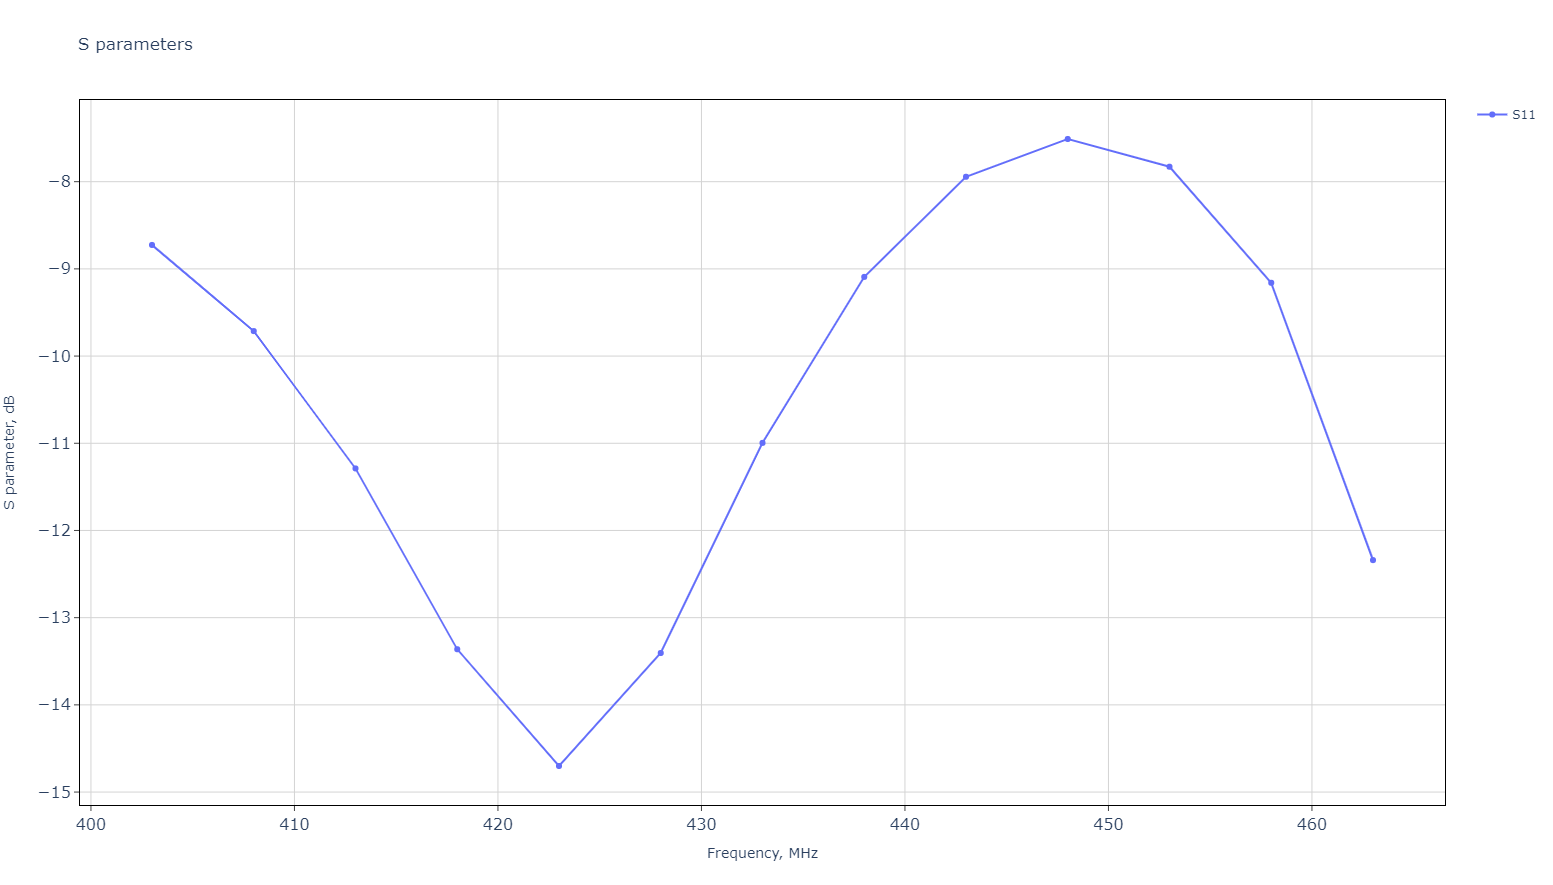
\includegraphics[width=10cm]{../ref/helix-naherung-S11.png}
	\label{fig:ersteHelixnäherung-S11}
	\caption{S11-Parameter der berechneten Helixantenne}
\end{figure}

\begin{figure}[h!]
	\centering
	\includegraphics[width=10cm]{../ref/helix-näherung-radiation-pattern.png}
	\label{fig:ersteHelixnäherung-abstrahldiagramm}
	\caption{Abstrahldiagramm der berechneten Helixantenne}
\end{figure}

Es wurde der Schluss gezogen, dass die Resonanzfrequenz zu weit unter dem gewünschten Wert von 433MHz liegt. Diese lässt sich durch Veränderung des Durchmessers der Spirale oder des Abstandes zwischen den Windungen verändern.

Durch das Abändern des Durchmessers konnte die gewünschte Resonanzfrequenz von 433MHz mit einem Helix-Durchmesser von 270mm erreicht werden. Der Reflektor wurde aus der Theorie mit ca. $\frac{3\lambda}{4}$ festgelegt \cite{Kraus-2002-AntennasB}, was einem Durchmesser von ungefähr 520mm entspricht.

\begin{figure}[H]
	\centering
	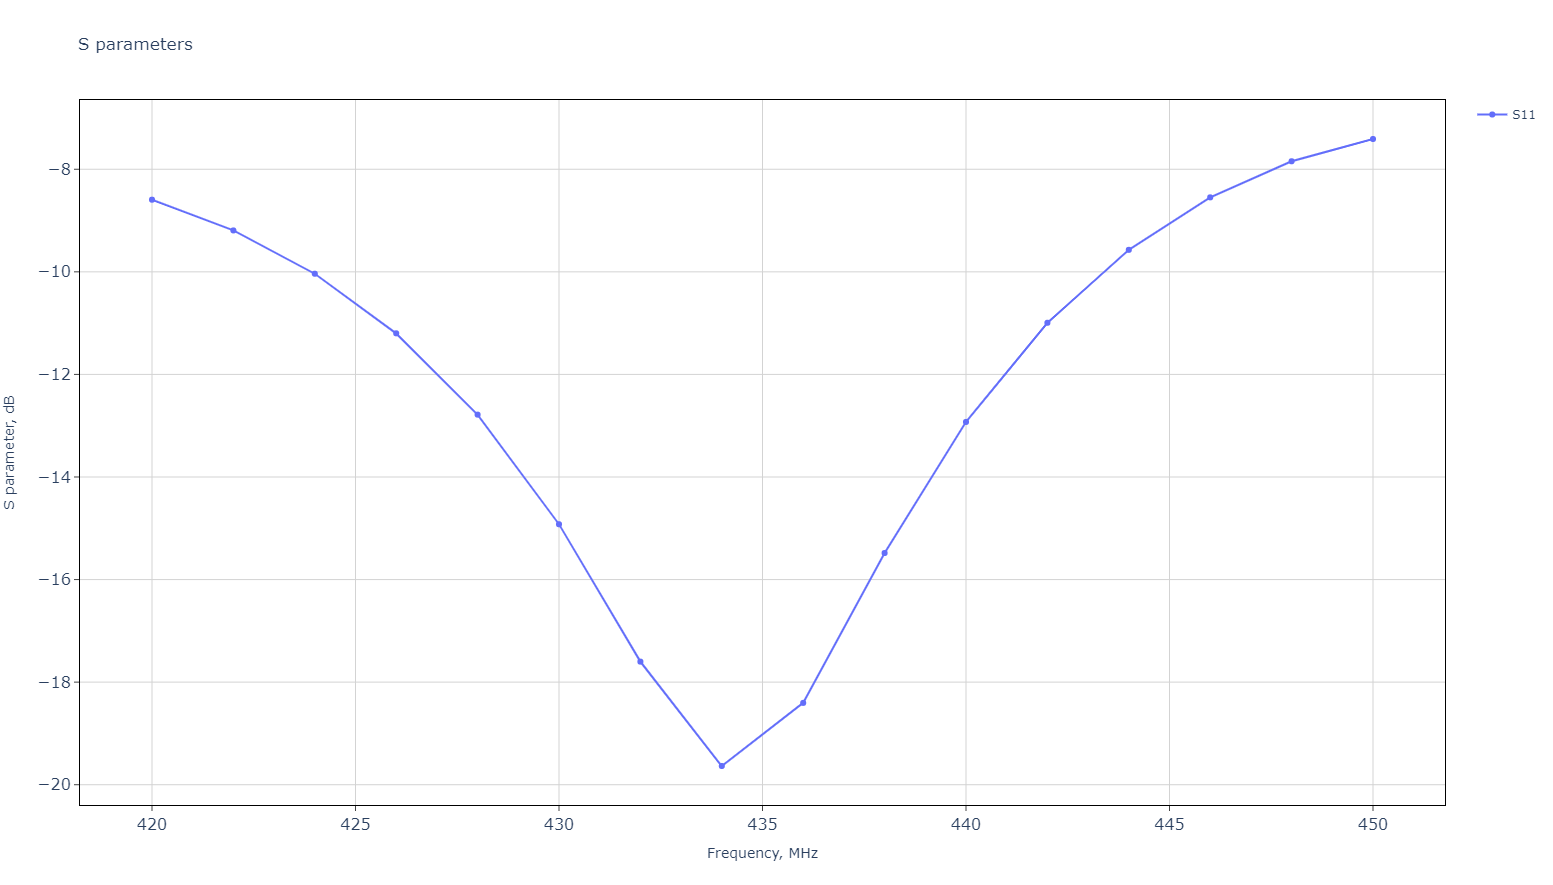
\includegraphics[width=10cm]{../ref/helix-fertig-S11.png}
	\label{fig:fertigeHelix-S11}
	\caption{S11-Parameter der richtig dimensionierten Helixantenne}
\end{figure}

\begin{figure}[H]
	\centering
	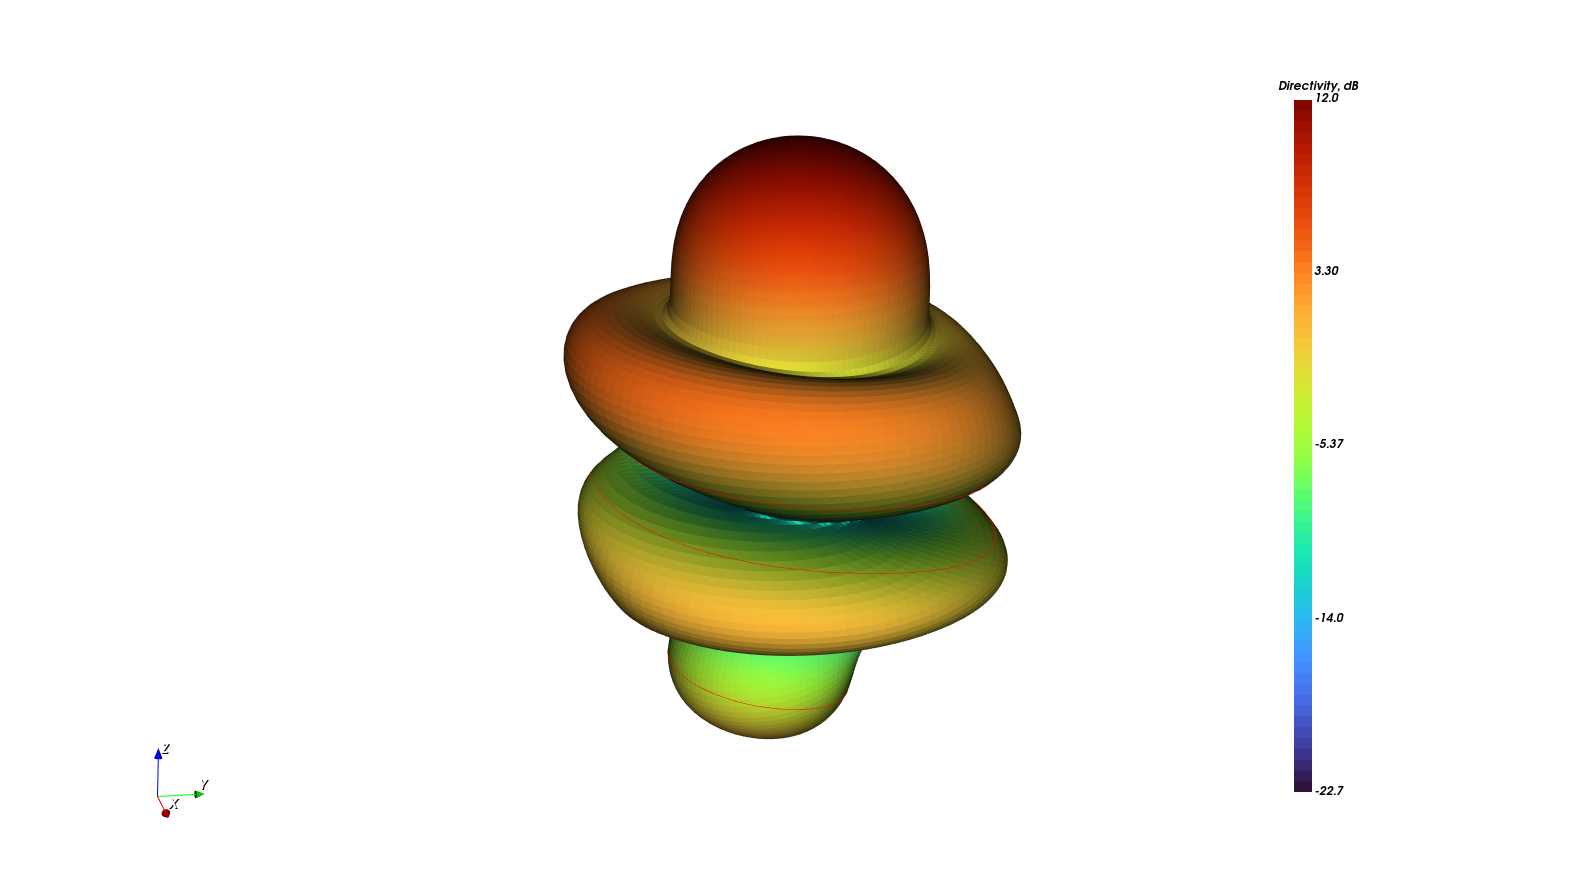
\includegraphics[width=10cm]{../ref/helix-fertig-radiation-pattern.png}
	\label{fig:fertigeHelix-Radiation}
	\caption{Abstrahldiagramm der richtig dimensionierten Helixantenne}
\end{figure}

Es ist wichtig anzumerken, dass der Steigungswinkel der Spirale hierbei ca. 11,5° beträgt. Dies hat zur Folge, dass die Steigung von dem relativ engen Idealbereich zwischen 12° und 14° abweicht.

\section{Realisierung}
Die Helixantenne benötigt zur Funktion nur zwei Bauteile: die Spirale und den Reflektor. Die Antenne funktioniert dann am Besten, wenn diese zwei Bauteile nicht von ihrer Umgebung beeinflusst werden. Hierfür muss darauf geachtet werden dass die Strukturelemente so wenig Kontakt mit der eigentlichen Antenne wie möglich haben. Um den Einfluss der Umgebung weiter zu verringern, werden spezielle Materialien mit einer niedrigen elektrischen Permittivität verwendet, beispielsweise Teflon, um kapazitive Einflüsse gering zu halten. 

\begin{figure}[H]
	\centering
	\includegraphics[width=10cm,angle=270]{../ref/Helixantenne-real.jpg}
	\caption{Reale Helixantenne}
	\label{fig:helix-real}
\end{figure}

\begin{table}
	\begin{tabular}{|c|c|c|c|c|}
	\hline
	Nr. & Typ & Maße & Besonderheiten & Menge \\
	\hline
	1 & PVC-Rohr & 50x3,7mm 1m & UV-stabilisiert & 4x \\
	\hline
	2 & Teflon-Rundlinge & \O 10mm 2m & UV-resistent & 4x \\
	\hline
	3 & PVC-Rohrschelle & toleriert 16-18mm & UV-stabilisiert & 44x \\
	\hline
	4 & Aluminiumrohr & 18x2mm 5,2m & & 4x \\
	\hline
	5 & Runde Aluminiumplatte & \O 520x3mm & & 4x \\
	\hline
	6 & Rohrflansch (Antenne) & \O innen 51mm &  & 4x \\
	\hline
	7 & Linsenkopf Kunststoffschrauben & M6x15mm &  & 44x \\
	\hline
	8 & Sechskant Kunststoffmuttern & M10 &  & 88x \\
	\hline
\end{tabular}
\caption{Stückliste für vier Helixantennen}
\end{table}

Auf dem PVC-Rohr wird die Helix der Antenne montiert, dieses ist UV-stabilisiert. Wäre der Kunststoff nicht gegen UV-Strahlung geschützt, so würde dieser nach einer Zeit spröde und strukturell unzuverlässig.

In das PVC-Rohr wurden Löcher mit einem Abstand von 86,6mm und einem Durchmesser von 11mm gebohrt. Diese schaffen genug Platz für die Seitenelemente welche einen Durchmesser von 10mm haben. Um das Rohr mithilfe des Rohrflansches an der Reflektorplatte zu montieren wurden zwei Löcher mit M10-Gewinde gebohrt.

Das gewählte Material ist PTFE, da es eine sehr niedrige elektrische Permittivität besitzt. Dies ist relevant, da die Spirale, welche die Resonanzfrequenz der Helixantenne bestimmt, so gut wie möglich von kapazitiven Einflüssen geschützt sein sollte. Das $\epsilon\textsubscript{r}$ von PTFE ist rund 2,2, während das von Luft ca. 1 ist \cite{lipinski_polytetrafluorethylen_nodate,noauthor_dielektrizitatskonstante_nodate}. Teflon ist zwar ein relativ weicher Kunststoff, allerdings ist Aluminium ein sehr leichtes Metall, welches durch die Teflonstäbe sicher gestützt werden kann. Da PTFE UV-beständig und ein allgemein widerstandsfähiger Kunststoff ist, eignet dieser sich bestens für den Einsatz im Freien.

\begin{figure}[H]
	\centering
	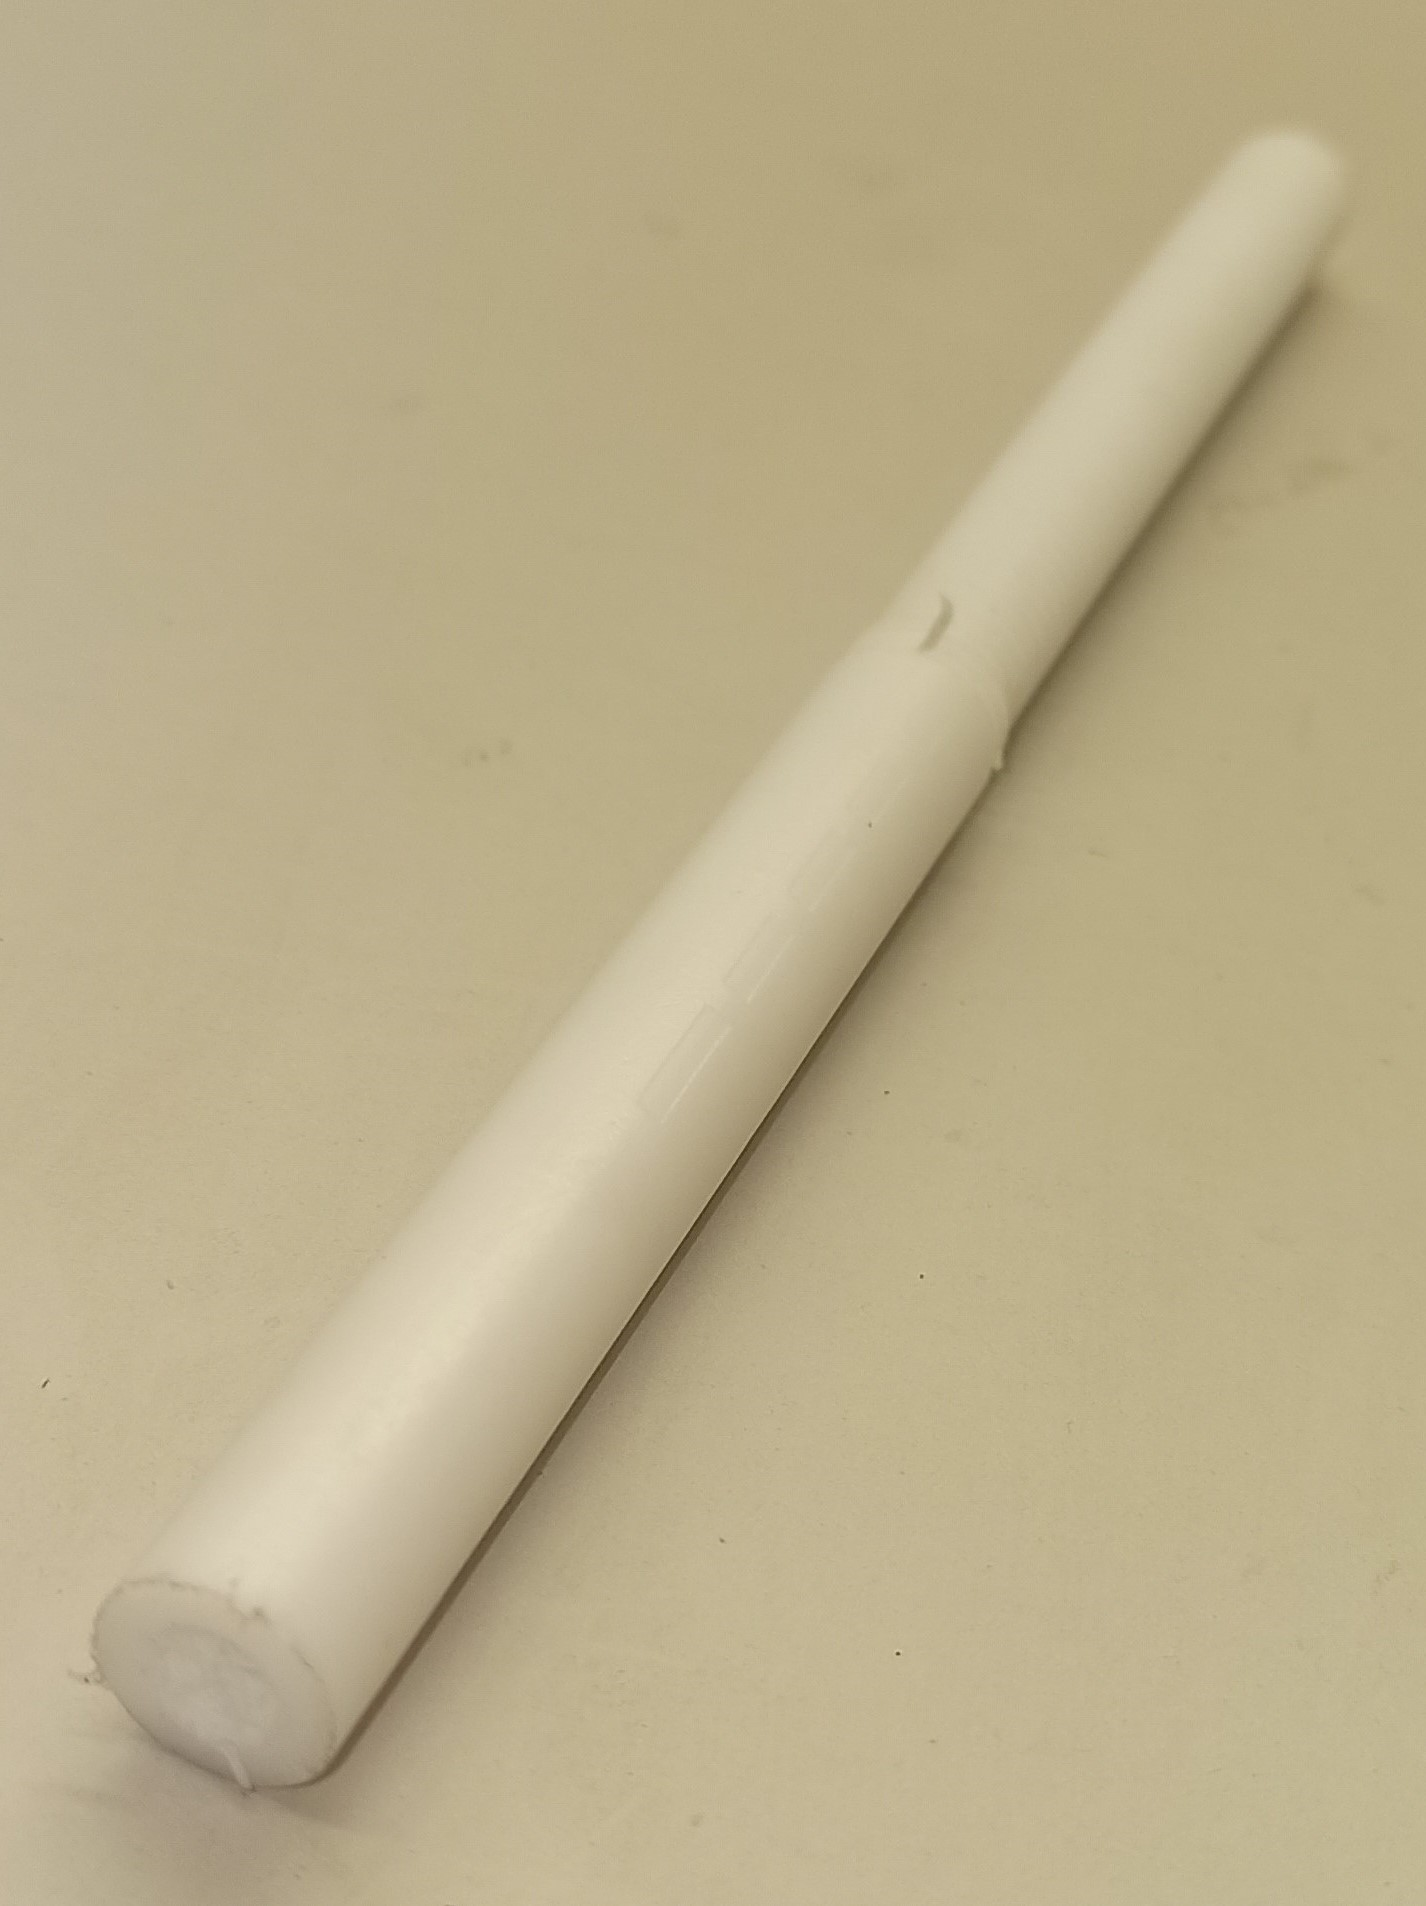
\includegraphics[width=5cm]{../ref/Abstandhalter-real.jpg}
	\label{fig:Abstandhalter-real}
	\caption{Realer Abstandhalter}
\end{figure}

Ein Abstandhalter ist ungefähr 150mm lang, das Außengewinde wird bis zur Hälfte der Teflonstange geschnitten. Der Stab wird mit dem Gewinde zuerst in die Löcher des PVC-Rohres gesteckt, damit dieser von vorne und hinten mit M10-Kunststoffmuttern an das Rohr geschraubt werden kann.

In die andere Seite des Abstandhalters wird ein Loch mit einem Durchmesser von 5mm für ein M6-Gewinde gebohrt. Mithilfe der entsprechenden Schrauben werden UV-stabilisierte Rohrschellen an dem Seitenelement montiert. Diese tolerieren Rohrdurchmesser von bis zu 18mm. Durch die Verwendung von Rohrschellen vereinfacht sich die Montage der Spirale auf ein einfaches Einschnappen des Rohres.

\begin{figure}[H]
	\begin{minipage}[b]{.4\linewidth} % [b] => Ausrichtung an \caption
		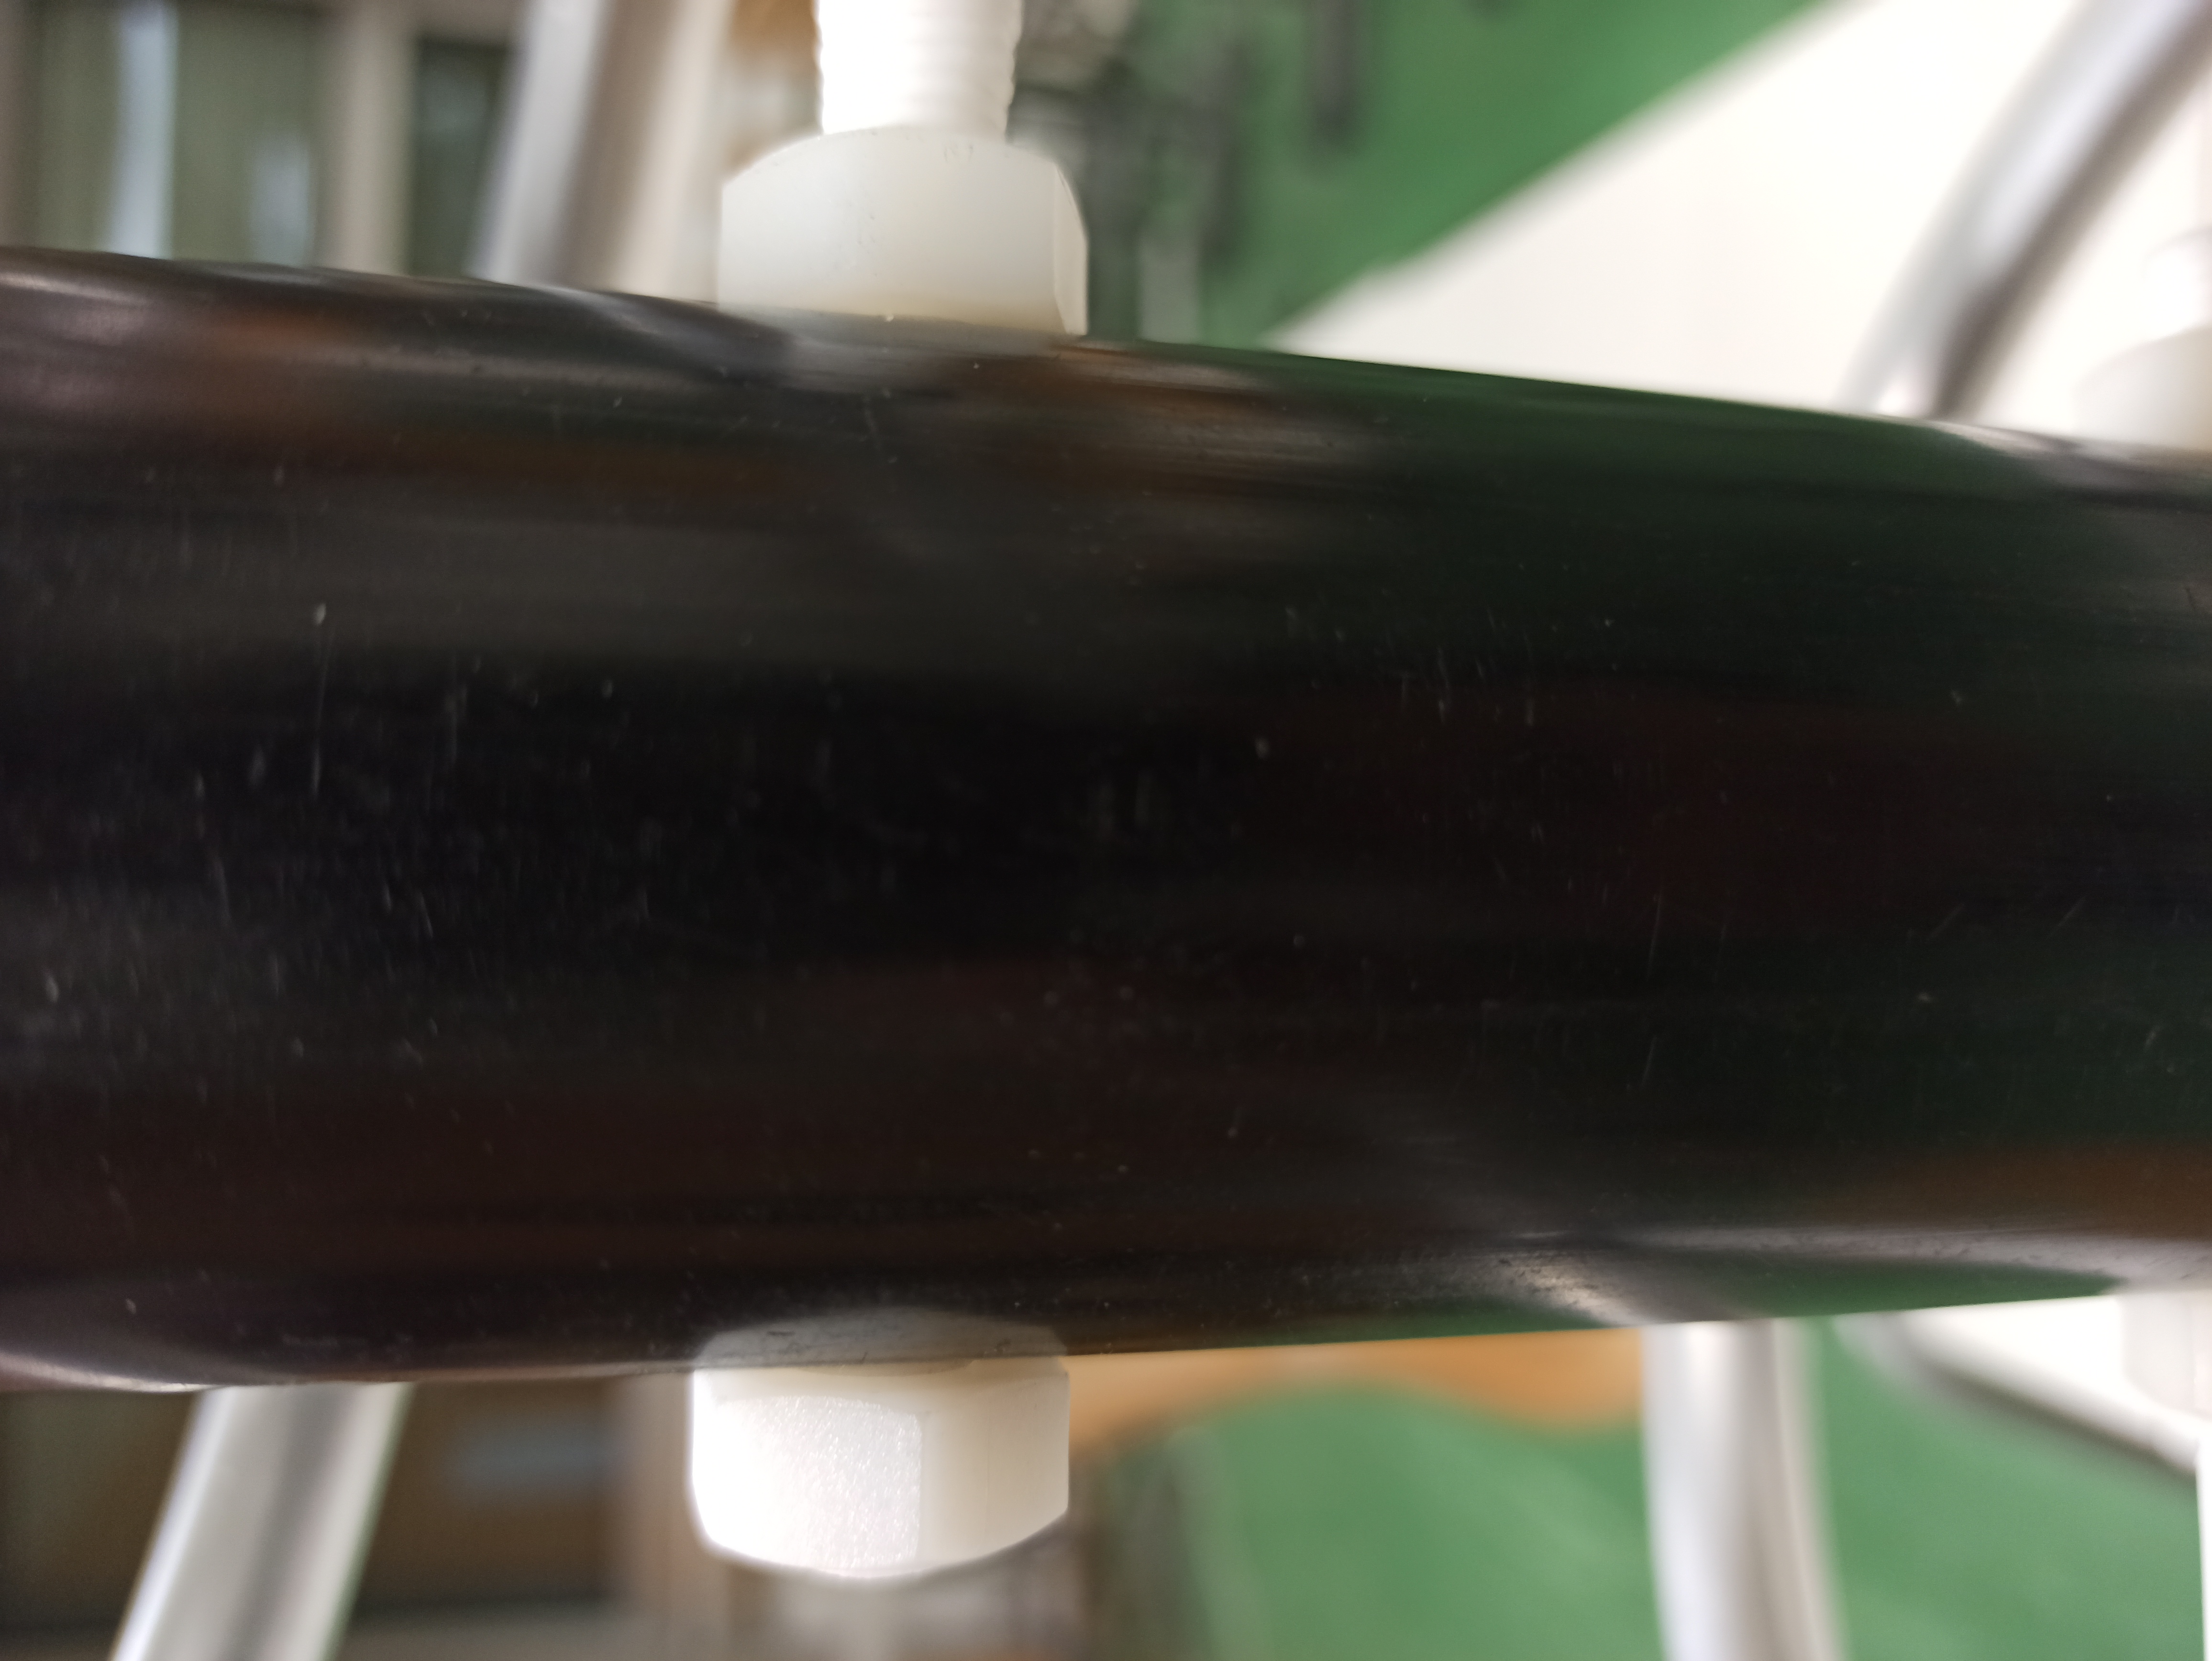
\includegraphics[width=7cm, angle=270]{../ref/Befestigung-Querelement.jpg}
		\label{fig:Abstandhalter-Befestigung}
	\end{minipage}
	\hspace{.1\linewidth}% Abstand zwischen Bilder
	\begin{minipage}[b]{.4\linewidth} % [b] => Ausrichtung an \caption
		\includegraphics[width=7cm, angle=270]{../ref/Rohrklemme-an-Spirale.jpg}
		\label{fig:Seitenelement-an-Spirale}
	\end{minipage}
	\caption{Links: Befestigung des Abstandhalters am Rohr. Rechts: Eingeschnappter Abstandhalter an der Spirale}
\end{figure}

Der Rohrflansch bildet das Bindeelement zwischen dem PVC-Rohr und der Reflektorplatte. Dieser hat einen Innendurchmesser von 51mm, und eine Wandstärke von 4mm. Es wird folglich 1mm an Toleranz geboten, damit das PVC-Rohr montiert werden kann. 

Der Rohrflansch besteht aus einem Rohr, in welches zwei durchgehende Löcher mit einem Durchmesser von 11mm gebohrt wurden, und einer Platte in die ebenfalls zwei Löcher mit einem Durchmesser von 13,5mm gebohrt wurden. Die Platte und das Rohr werden aneinander geschweißt. Das resultierende Bauteil bildet das Bindeglied zwischen Reflektor und PVC-Rohr.

Für den Reflektor wurde eine runde Aluminiumplatte gewählt. Für die reale Konstruktion wurden Löcher in den äußeren Rand der Platte gelasert, um den Luftwiderstand zu reduzieren. Um eventuelle Störungen durch spezifische Maße wie beispielsweise $\frac{\lambda}{4}$ zu vermeiden, wurden die Löcher um einiges kleiner als dieses Maß dimensioniert.

\begin{figure}[H]
	\begin{minipage}[b]{.4\linewidth} % [b] => Ausrichtung an \caption
		\includegraphics[angle=270,width=\linewidth]{../ref/Rohrflansch-Antenne.jpg}
		\label{fig:Rohrflansch-Antenne-Verbindung}
	\end{minipage}
	\hspace{.1\linewidth}% Abstand zwischen Bilder
	\begin{minipage}[b]{.4\linewidth} % [b] => Ausrichtung an \caption
		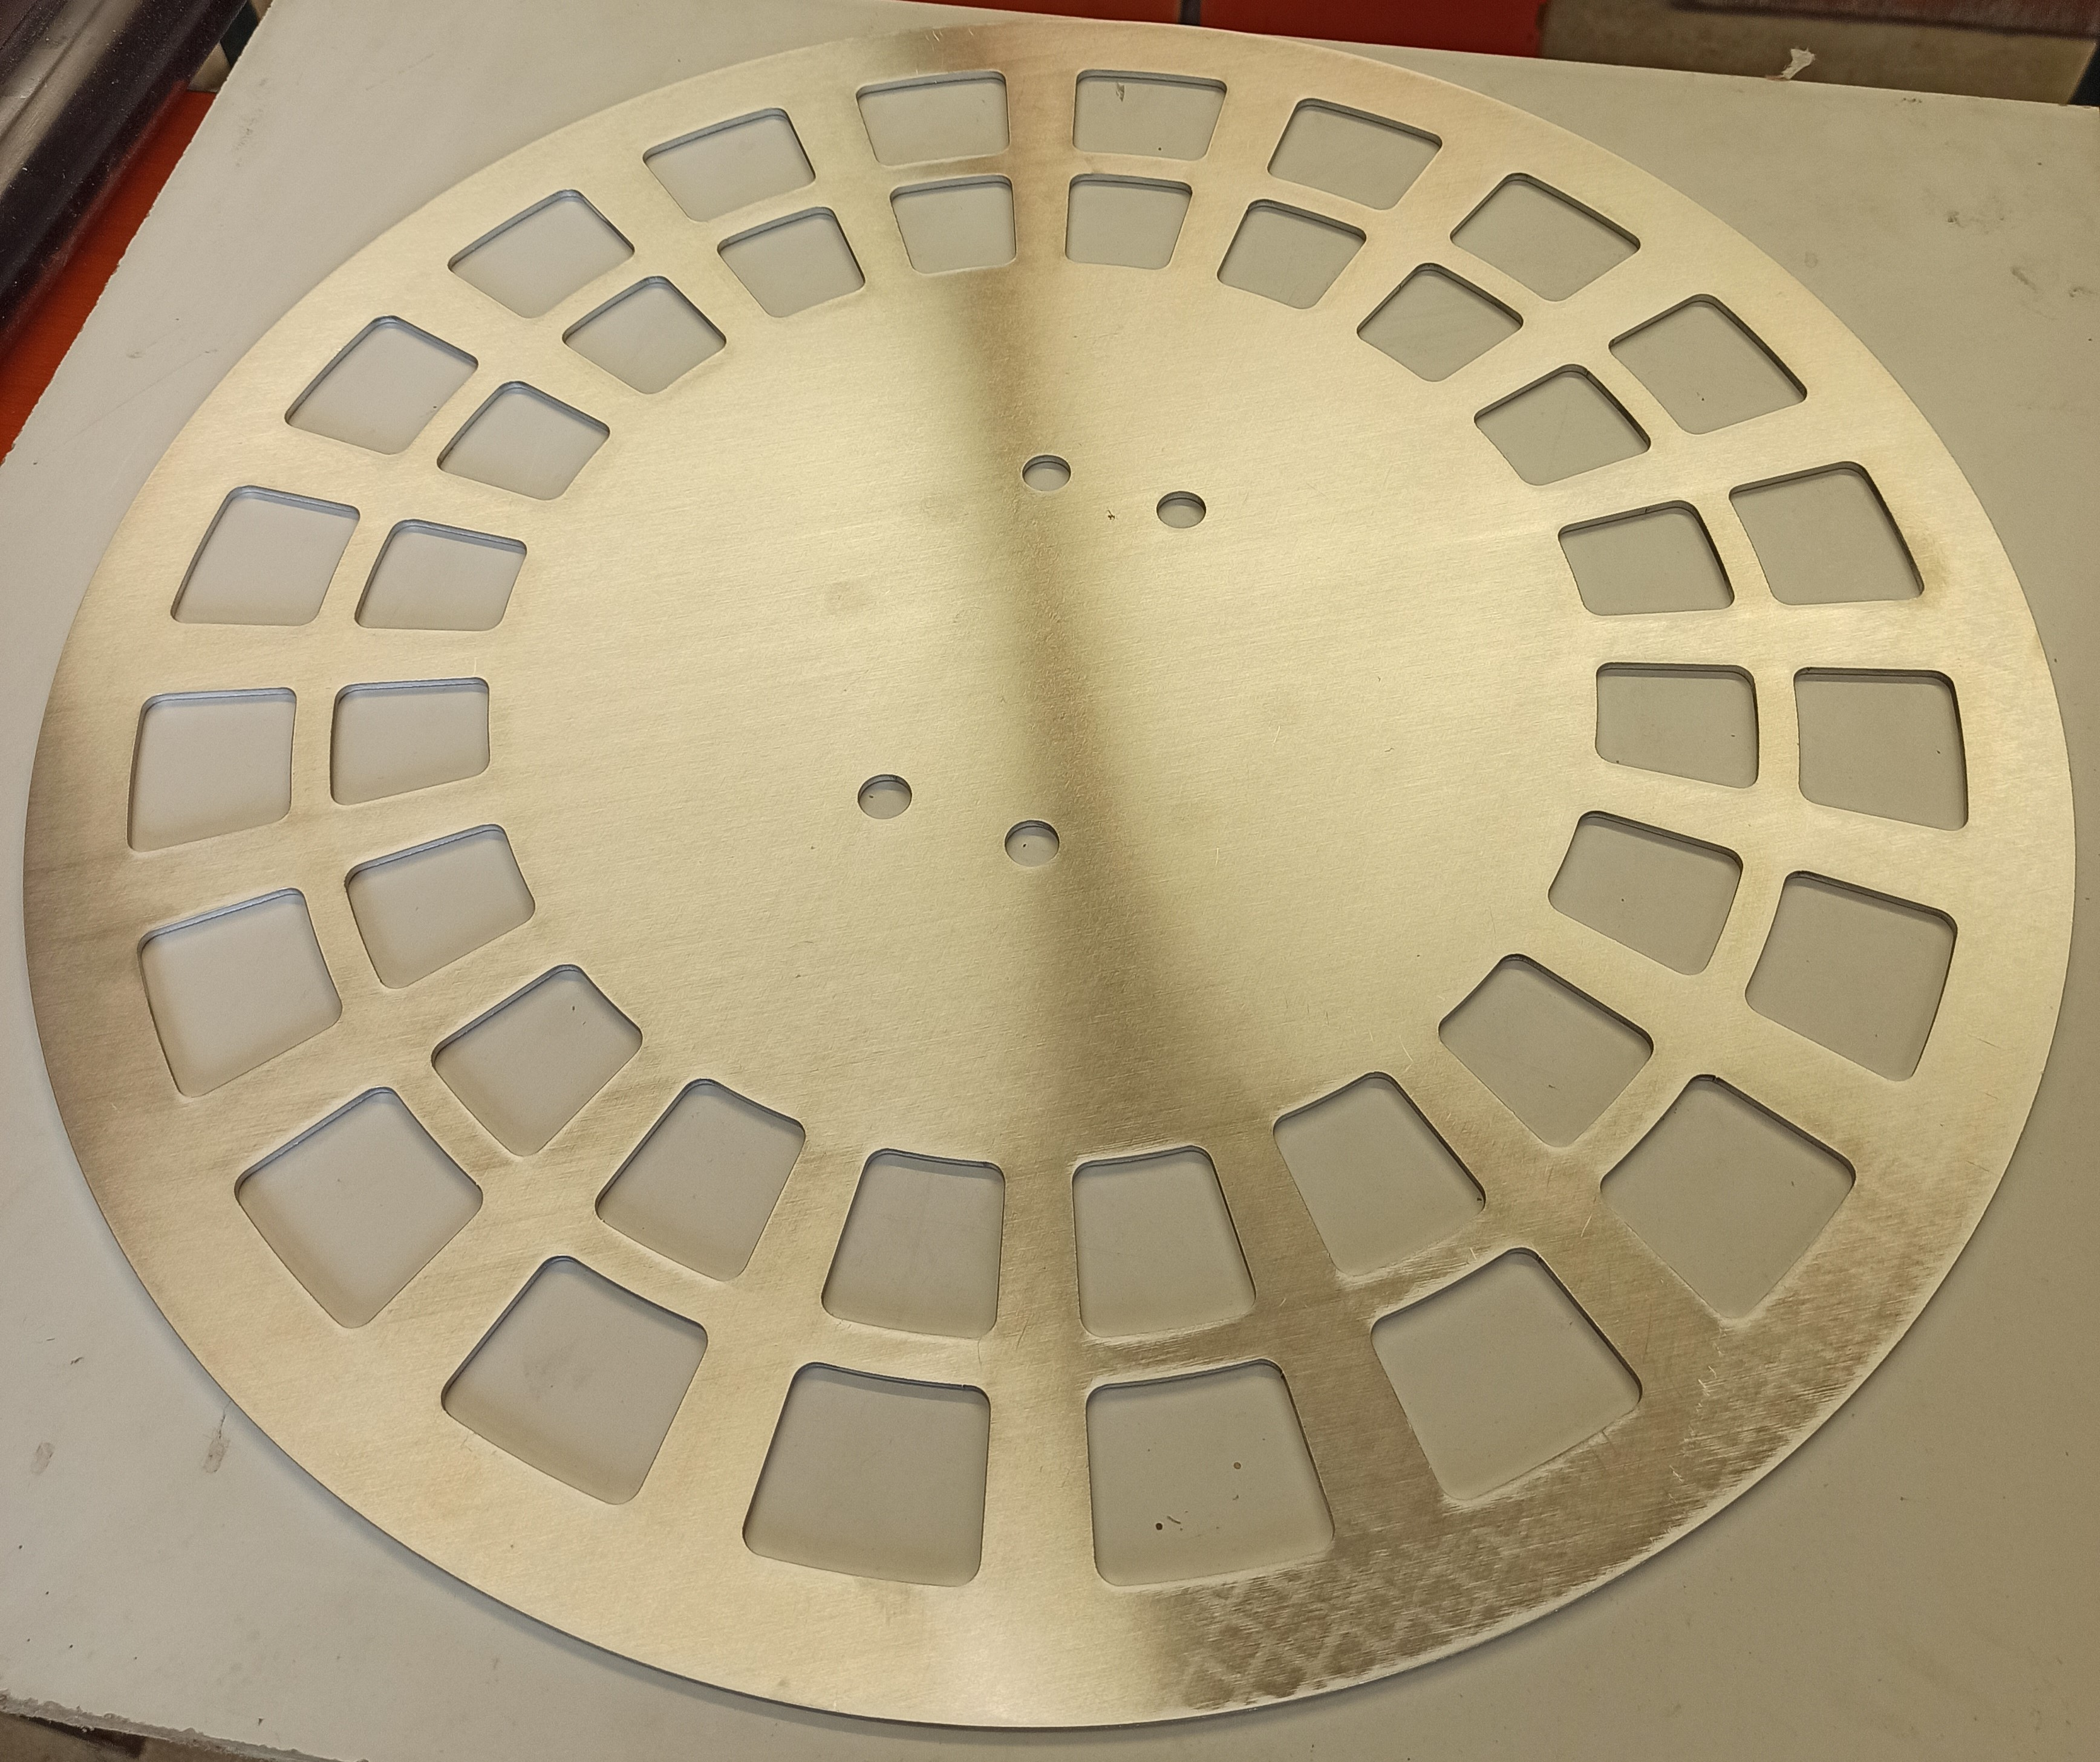
\includegraphics[width=\linewidth]{../ref/Reflektor.jpg}
		\label{fig:Reflektor}
	\end{minipage}
	\caption{Reflektor (rechts) im Vergleich mit dem daran befestigten Rohrflansch (links)}
\end{figure}

In der Mitte des Reflektors werden vier Löcher mit einem Durchmesser von 13,5mm gebohrt an denen der Rohrflansch befestigt wird. 

Die Helix wurde mit denselben Maßen gefertigt, welche in der Simulation ermittelt wurden. Hierfür wurde ein Aluminiumrohr verwendet, welches zu einer Spirale gebogen wurden die einen Durchmesser von 270mm, eine Höhe von ca. 1039,2mm und konsequent eine Steigung von 11,5° beziehungsweise einen Abstand zwischen den Windungen von 173,2mm ($\frac{\lambda}{4}$) hat.

\begin{figure}[h!]
	\centering
	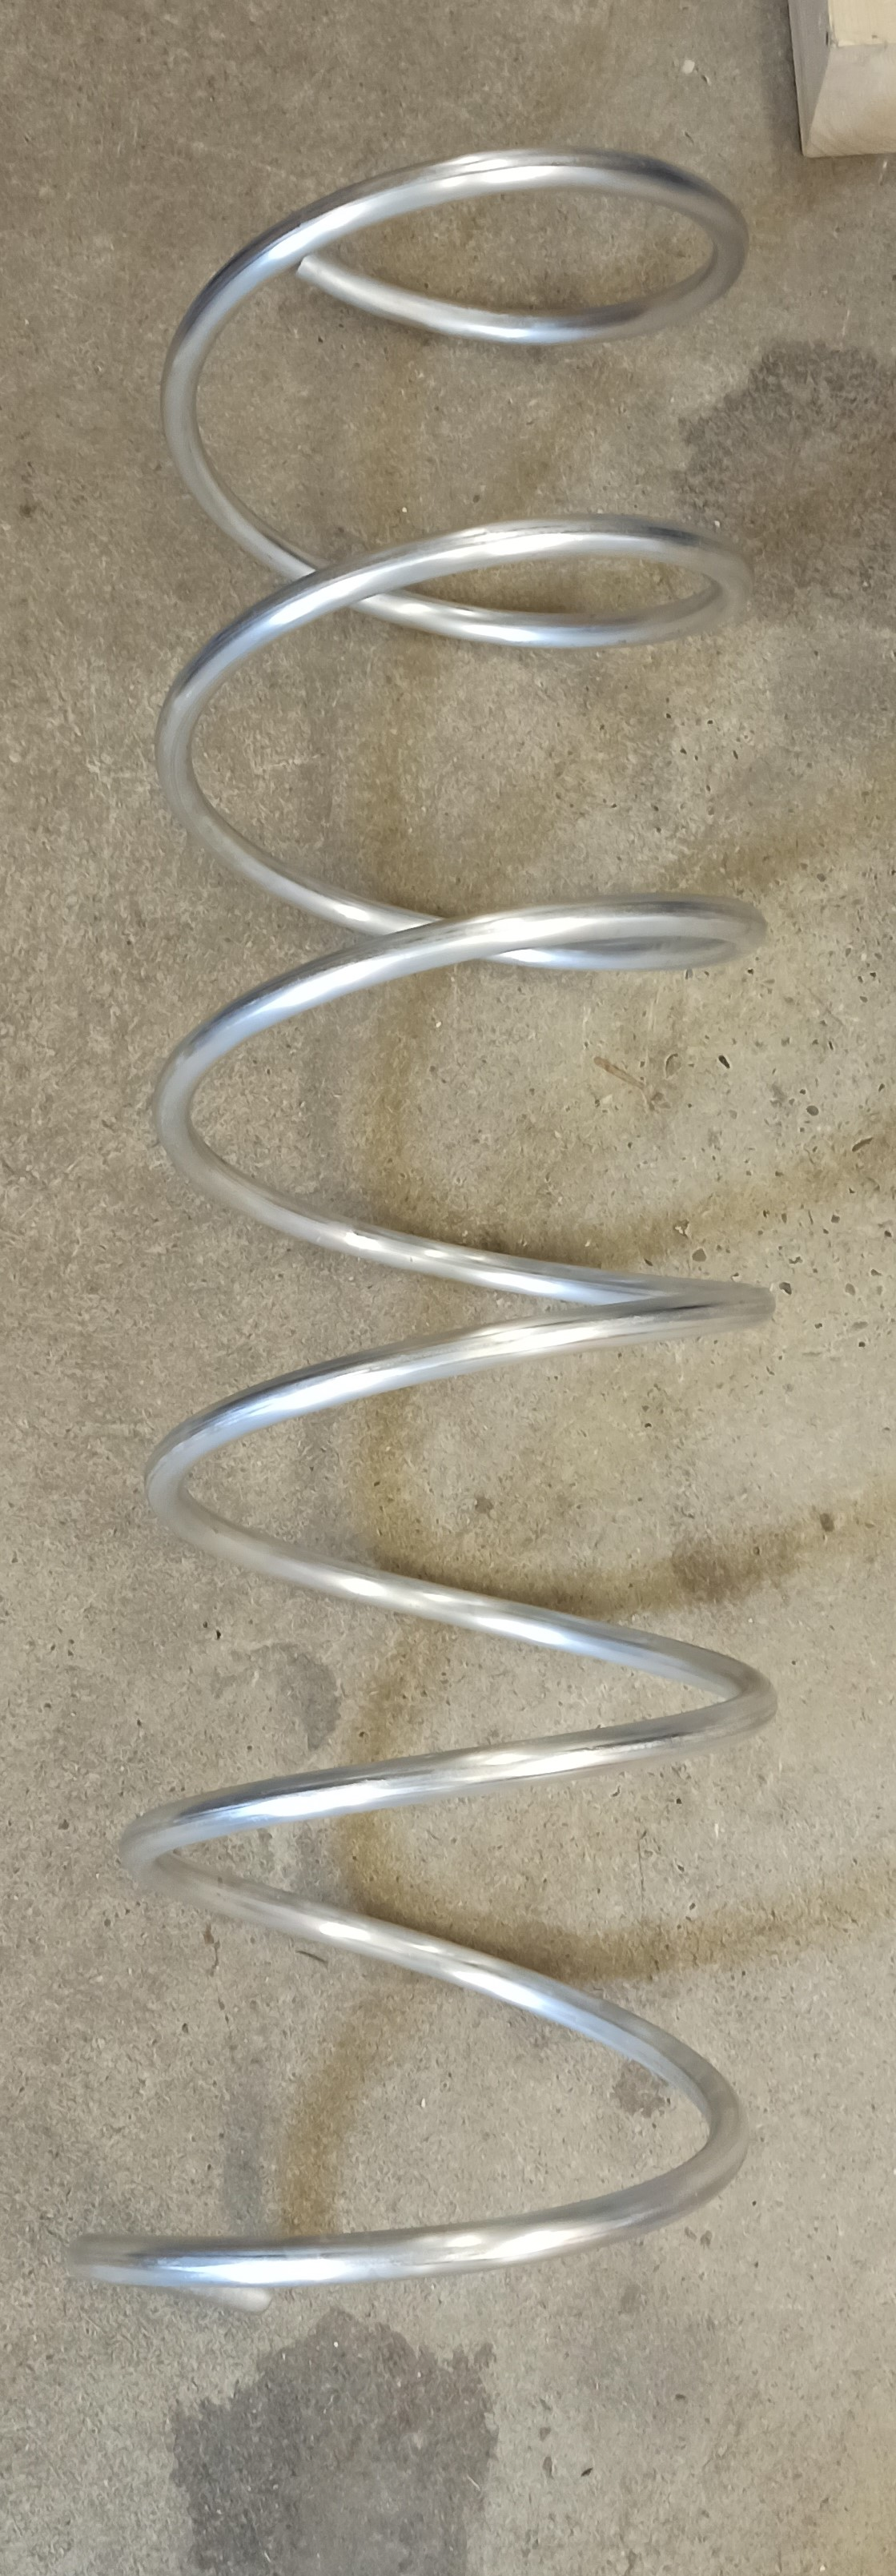
\includegraphics[width=5cm,angle=90]{../ref/Spirale.jpg}
	\caption{Die Spirale}
	\label{fig:Spirale}
\end{figure}

Um die Helixantenne wasserdicht zu machen wurden kurz abgeschnittene Aluminium-Rundlinge auf die Öffnungen der Spirale geschweißt. Am unteren Ende der Helix, an der der Innenleiter des Koaxialkabels befestigt wird, wurde ein Gewinde in den Aluminium-Rundling geschnitten.

\begin{figure}[h!]
	\begin{minipage}[b]{.4\linewidth} % [b] => Ausrichtung an \caption
		\includegraphics[width=\linewidth]{../ref/Deckel-oben.jpg}
		\label{fig:Deckel-Helix-Oben}
	\end{minipage}
	\hspace{.1\linewidth}% Abstand zwischen Bilder
	\begin{minipage}[b]{.4\linewidth} % [b] => Ausrichtung an \caption
		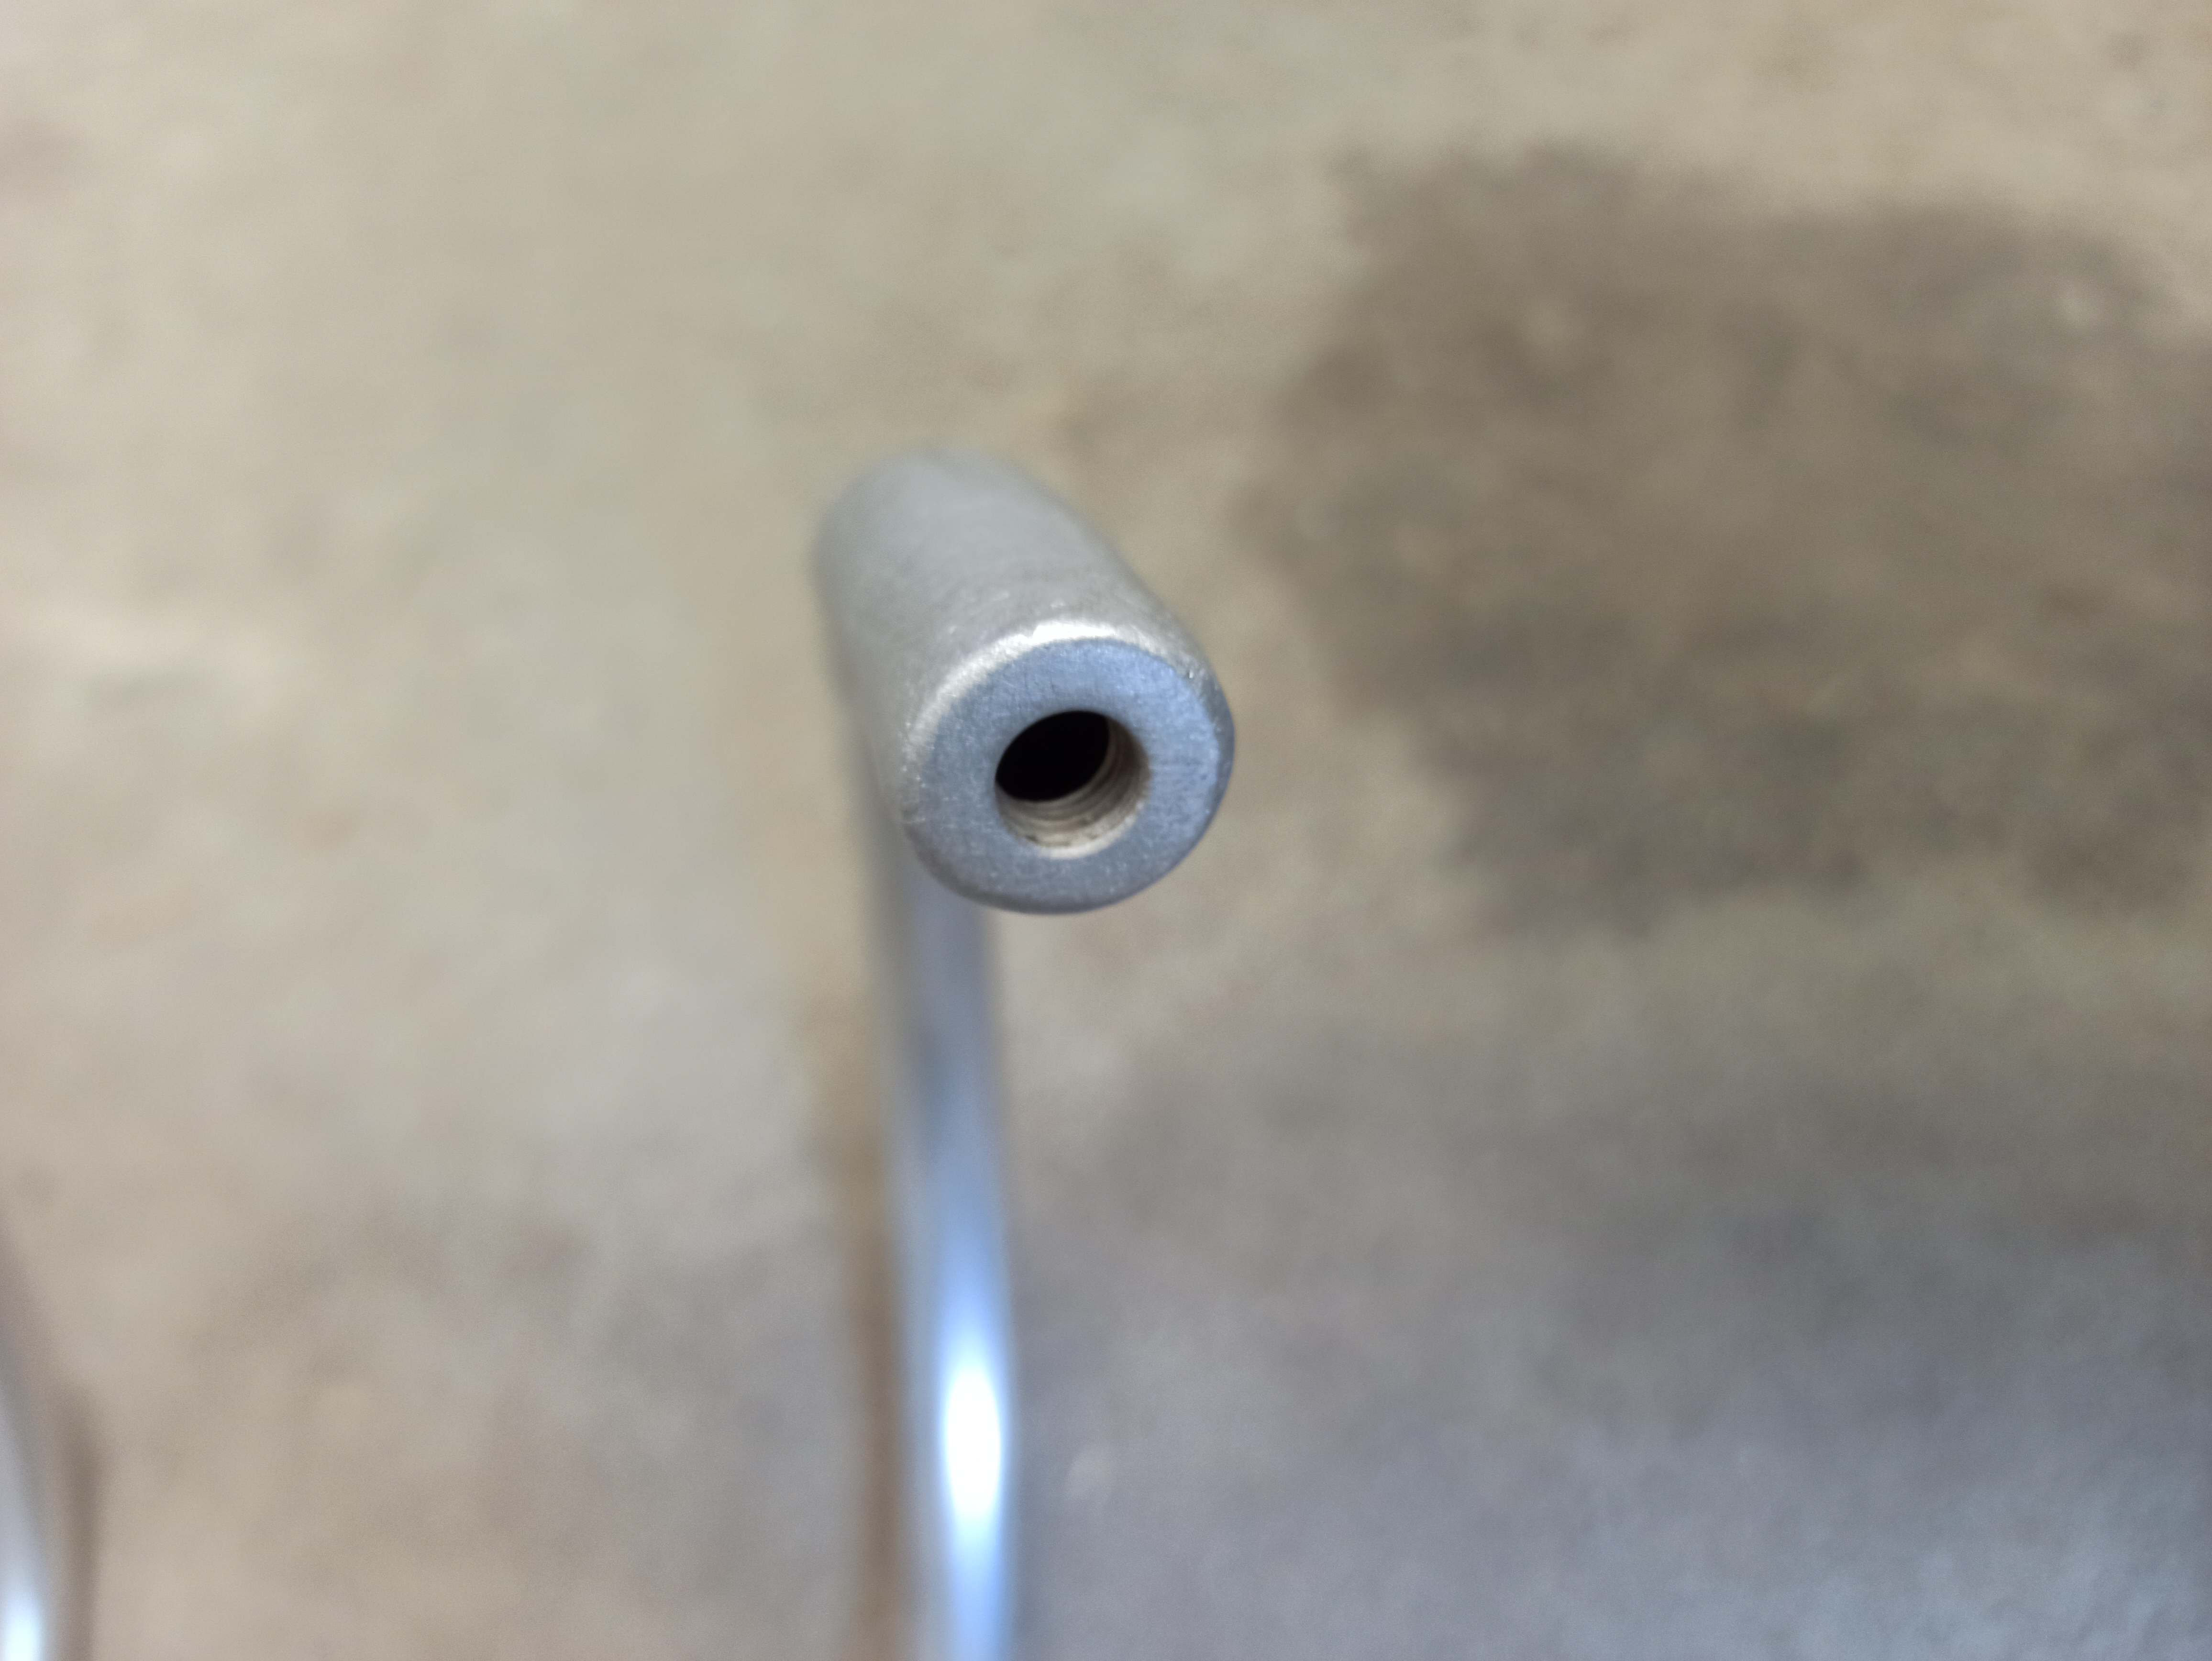
\includegraphics[width=\linewidth]{../ref/Anschluss-unten.jpg}
		\label{fig:Deckel-Helix-Unten}
	\end{minipage}
	\caption{Links: Zugeschweißtes oberes Ende der Helix.Rechts: Gewinde am unteren Ende der Helix zur Anbringung des Innenleiters}
\end{figure}

Mithilfe dieses Gewindes kann ein Kabel durch eine Schraube montiert, und am Innenleiter der BNC-Buchse angelötet werden.

Um die PVC-Rohre vor Wasser zu schützen wurden Abdeckungen 3D-gedruckt. Durch die Verwendung eines speziellen Filaments vom Typ DuraPro ASA, ist das Resultat eine UV-resistente Rohrabdeckung. Durch diese Eigenschaft eignet sich dieses Filament exzellent für den Einsatz im Freien.

\begin{figure}[H]
	\centering
	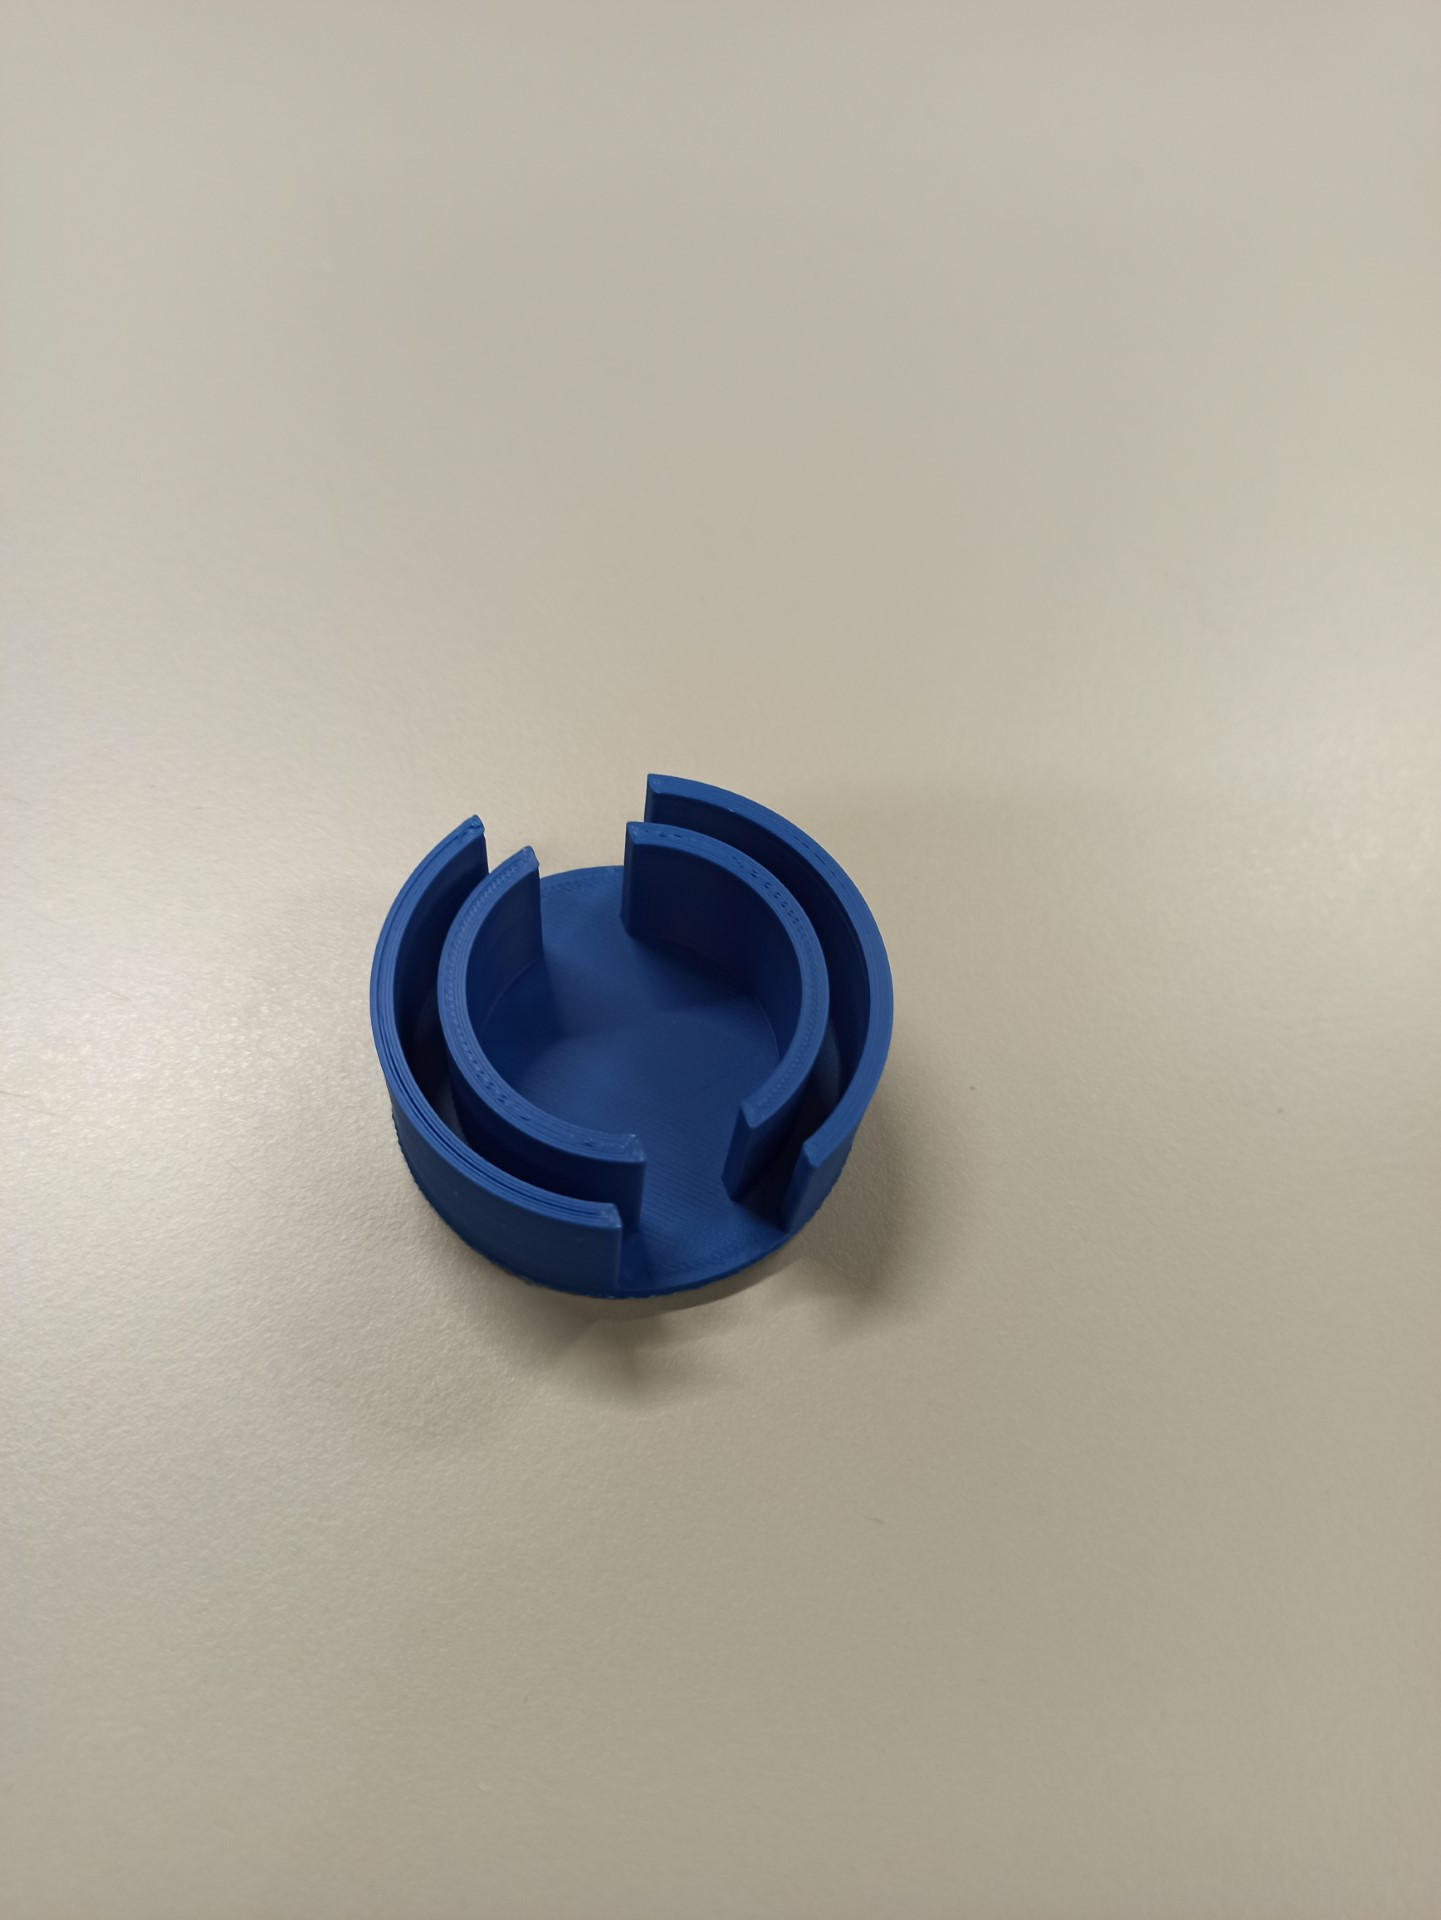
\includegraphics[width=5cm]{../ref/Abdeckung-PVC-Rohr.jpg}
	\caption{Die Abdeckung des PVC-Rohres}
	\label{fig:PVC-Rohr-Abdeckung}
\end{figure}

Die BNC-Buchse befindet sich direkt unter dem Ende der Spirale. Der Innenleiter wird, wie bereits erwähnt, an der Helix befestigt. Der Außenleiter wird mit dem Reflektor verschraubt.

\begin{figure}[H]
	\begin{minipage}[b]{.4\linewidth} % [b] => Ausrichtung an \caption
		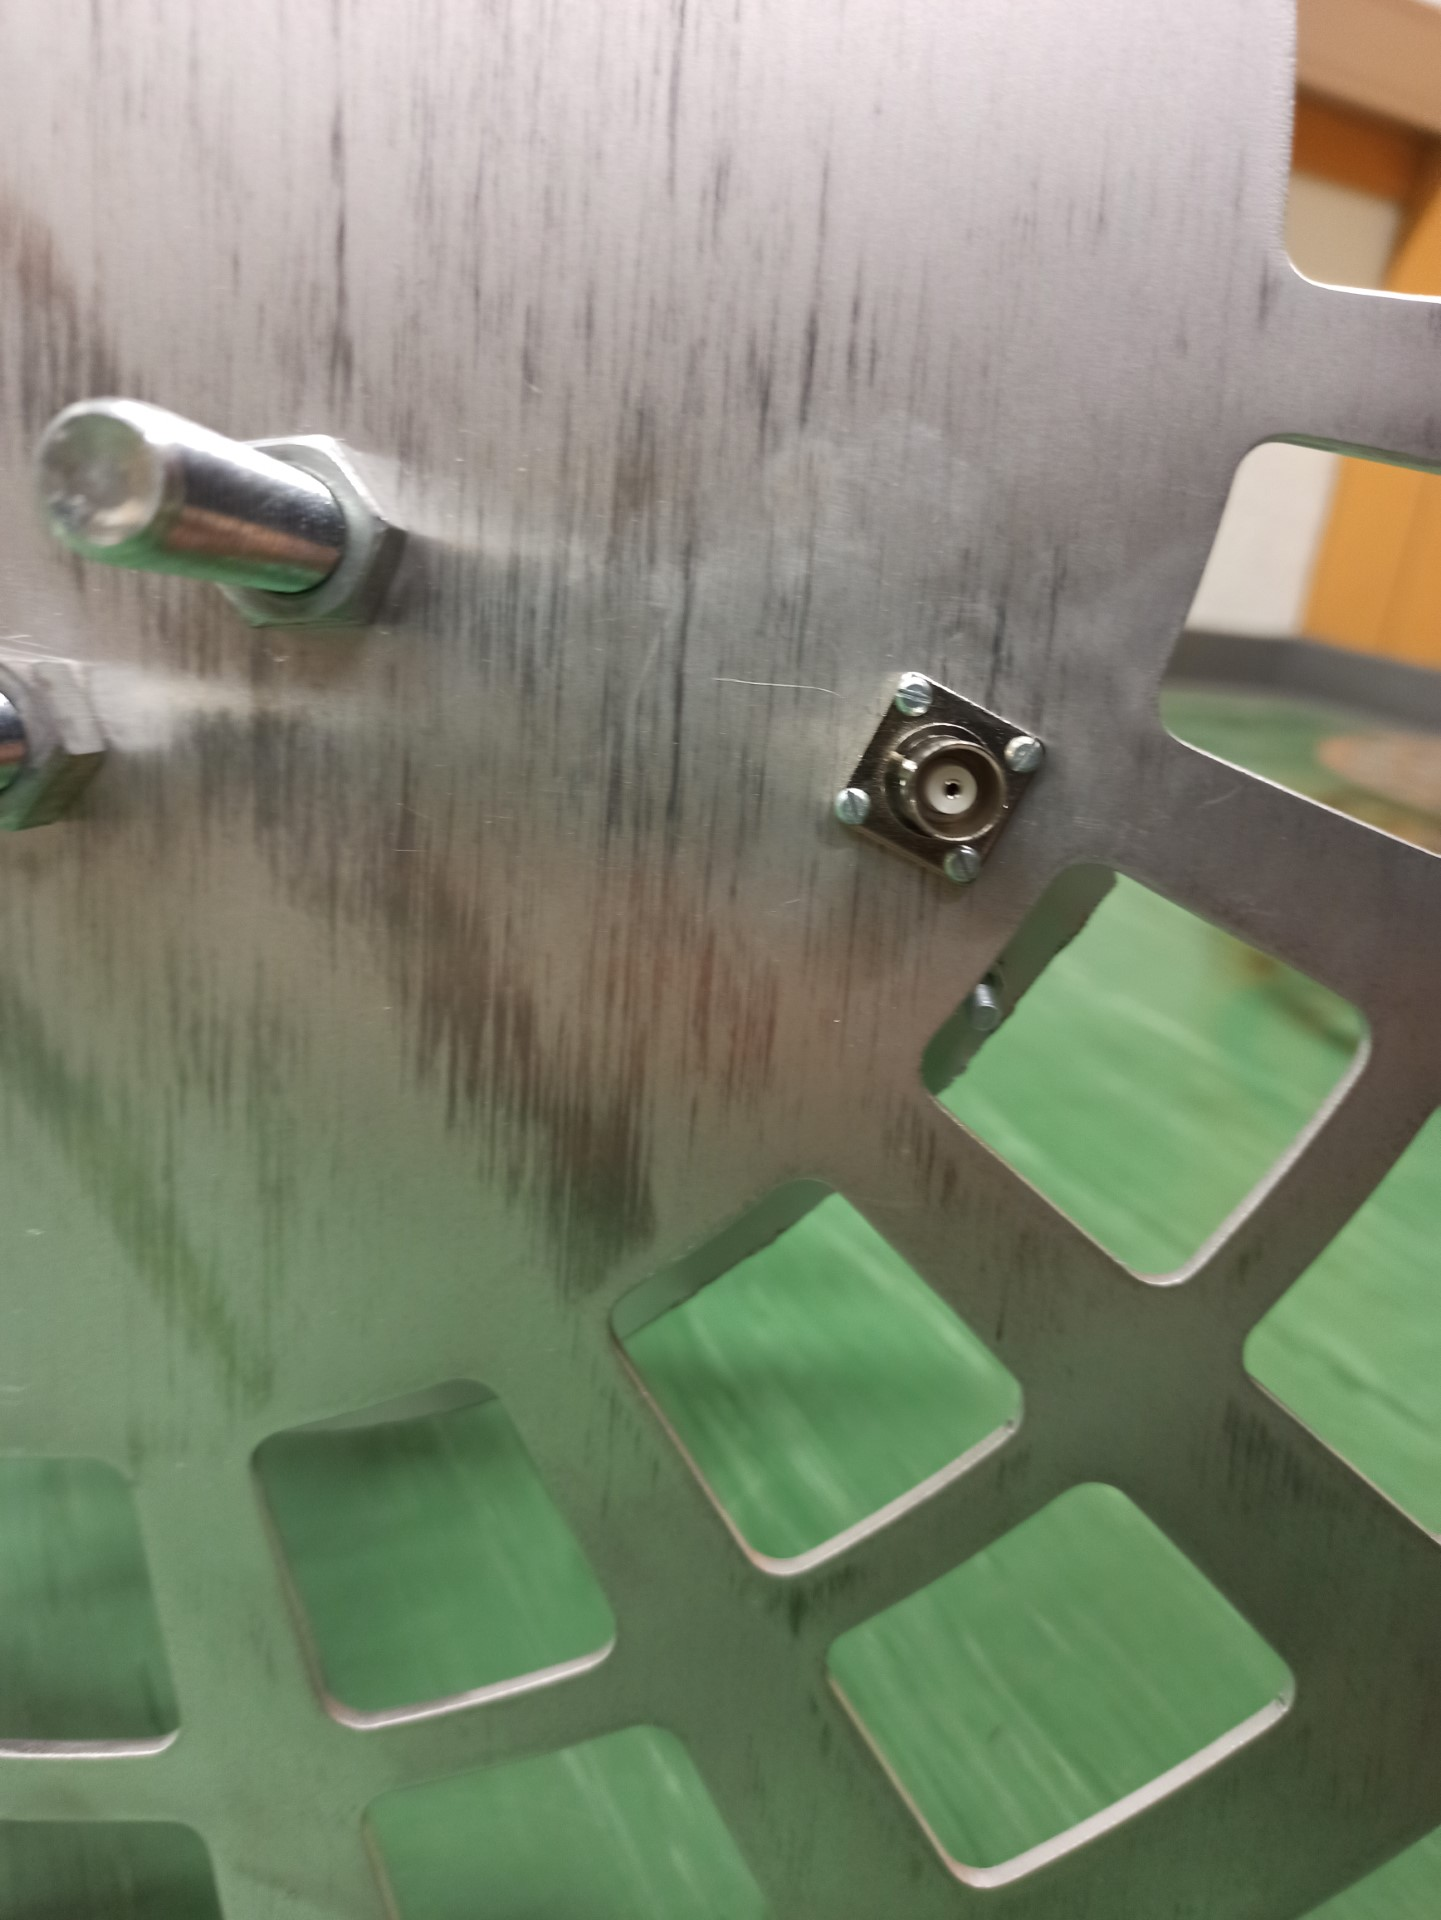
\includegraphics[width=\linewidth]{../ref/BNC-Buchse.jpg}
		\label{fig:BNC-Buchse}
	\end{minipage}
	\hspace{.1\linewidth}% Abstand zwischen Bilder
	\begin{minipage}[b]{.4\linewidth} % [b] => Ausrichtung an \caption
		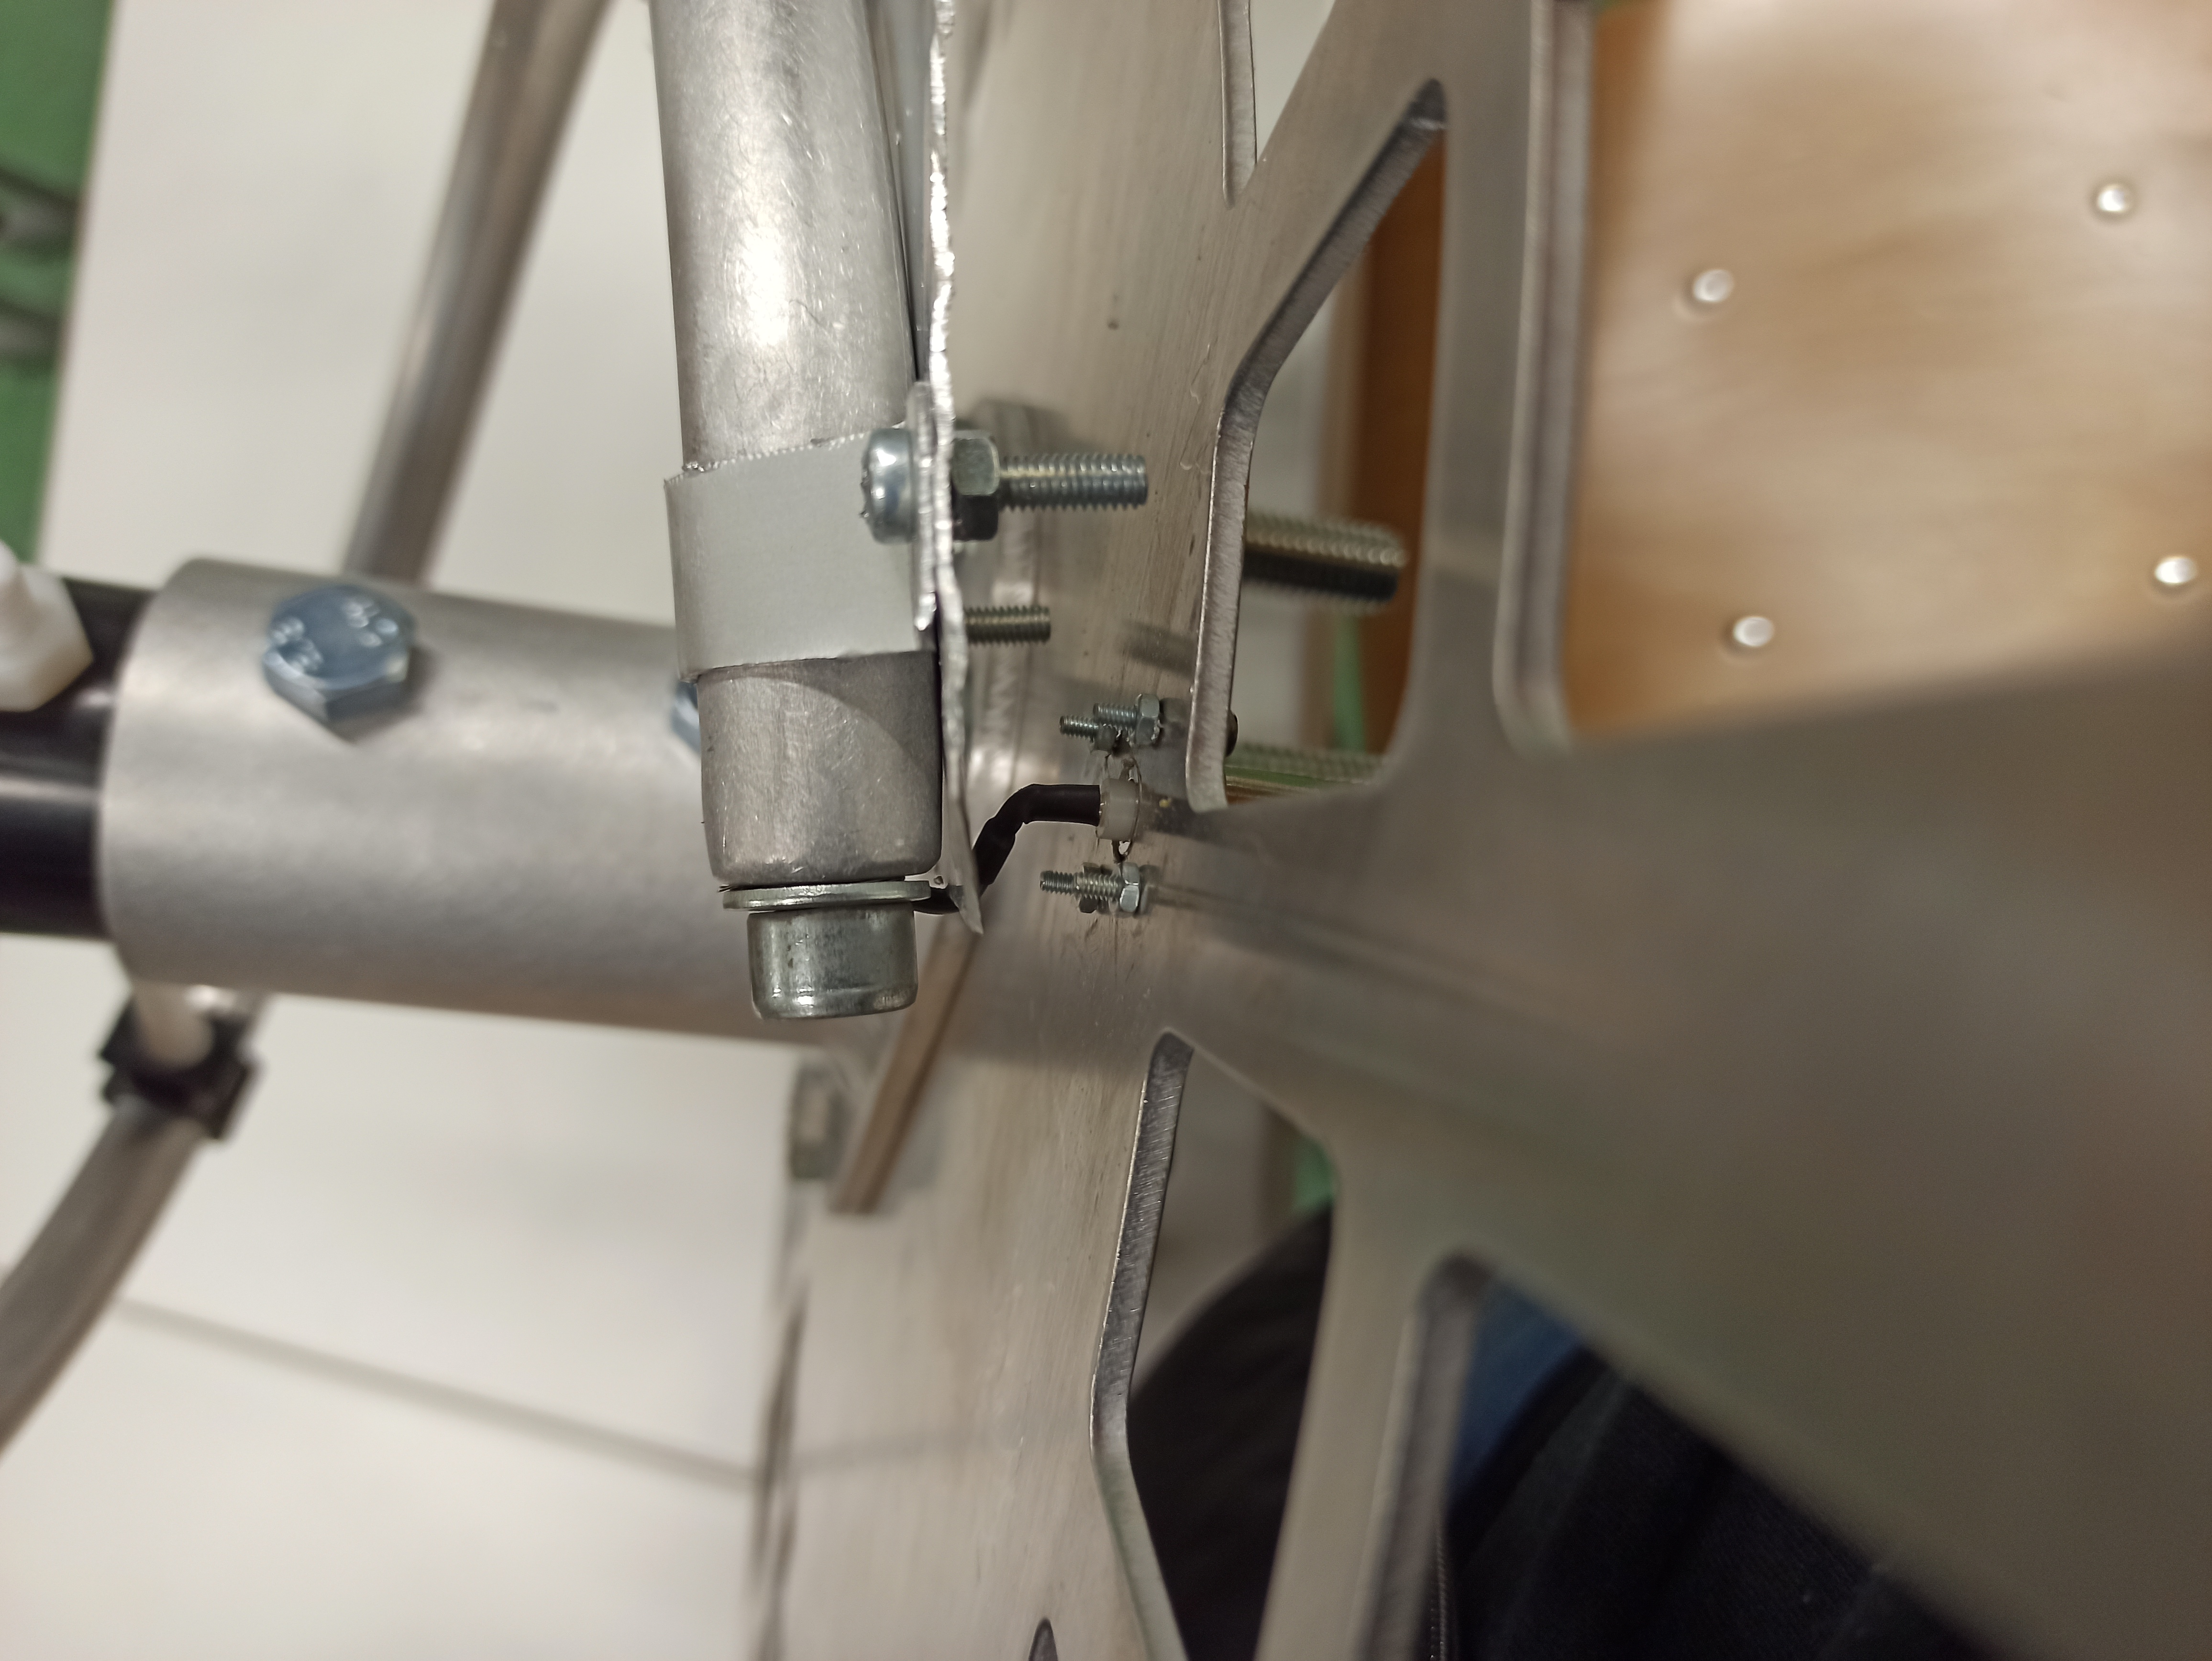
\includegraphics[angle=270,width=\linewidth]{../ref/Befestigung-Innenleiter.jpg}
		\label{fig:Innenleiter-Befestigung}
	\end{minipage}
	\caption{Koaxialkabel-Anschluss}
\end{figure}

\section{Anpassung}
Um eine einzelne Helixantenne anzupassen gibt es verschiedene Möglichkeiten. Eine weit verbreitete Option ist es, einen entsprechend dimensionierten Blechstreifen mit einer Länge von $\frac{\lambda}{4}$ entlang des unteren Endes der Helix zu montieren. Dieser agiert als Resonanztransformator und soll die Impedanz der Antenne auf einen Wert von 50$\Omega$ senken \cite{kgwadi_parametric_2014}.

\begin{figure}[H]
	\centering
	\includegraphics[width=7cm]{../ref/Anpassstreifen.jpg}
	\caption{Der realisierte Blechstreifen für die Impedanzanpassung}
	\label{fig:matching-strip}
\end{figure}

Die Breite des Blechstreifens wurde empirisch ermittelt und wurde mit 6cm festgelegt. Um den S11-Parameter auf einen akzeptablen Wert zu bringen, wird der Abstand zwischen Reflektor und Spirale verringert. Dadurch beeinflussen sich der Blechstreifen und die auf Masse liegende Reflektorplatte auf eine Weise, die die Performance der Antenne steigert.

\section{Erweiterung der Helixantenne als Array}
Nun wird die Helixantenne durch drei weitere identische Helixantennen erweitert, welche zusammen ein Array bilden. Hierbei ist der Abstand zwischen den einzelnen Antennen von Relevanz um den Gesamtgewinn zu maximieren.
Der Antennengewinn eines Antennenarrays bestehend aus vier identischen Helixantennen liegt in der Theorie bei dem vierfachen Antennengewinn einer einzelnen Wendelantenne, bzw. einer Helixantenne mit der vierfachen Windungszahl, also $4*6=24$ \cite[p. 319]{Kraus-2002-AntennasB}.

\begin{figure}[h!]
	\centering
	\includegraphics[angle=270,width=5cm]{../ref/Antennenarray2.jpg}
	\caption{Das fertige Helixantennen-Array}
	\label{fig:helixantennen-array}
\end{figure}

Hierfür muss ein Gerüst designt und aufgebaut werden, welches vier solcher Antennen halten kann, sowie die neu entstehende Impedanz der Zusammenschaltung dieser Antenne angepasst werden. Anschließend müssen Tests durchgeführt werden, die den verbesserten Antennengewinn der Antenne belegen.

\subsection{Gerüst}
\label{subsec:helix_geruest}
\begin{table}
	\begin{tabular}{|c|c|c|c|}
	\hline
	Nr. & Typ & Maße & Menge \\
	\hline
	1 & Aluminiumrohr & \O42x2,5mm 0,77m & 1x \\
	\hline
	2 & Aluminium-Vierkantrohr & 60x100x3mm 0,9m & 2x \\
	\hline
	3 & Rohrflansch (Struktur) & \O innen 45mm & 2x\\
	\hline
	4 & Zylinderkopfschraube & \O M12x80mm & 4x\\
	\hline
	5 & Sechskantschraube & \O M10x20mm & 24x\\
	\hline
	6 & Linsenkopfschraube & \O M5x10mm & 16x\\
	\hline
\end{tabular}
\caption{Stückliste Gerüst}
\end{table}

Als Gerüst wurde die Form eines $"$H$"$ gewählt. Hierdurch liegt der Massenmittelpunkt der Gesamtkonstruktion nur knapp über dem Mittelpunkt des Rotors, was das zur Rotation benötigte Moment verringert. Um dies zu beweisen lässt sich die Formel für das mechanische Moment betrachten.
\begin{equation}
	M=F*r*\sin(\alpha)
	\label{form:drehmoment}
\end{equation}
Hierbei ist r die Länge des Hebels, und in diesem Kontext der Abstand des Schwerpunktes der Konstruktion zum Mittelpunkt. Je näher der Schwerpunkt am Mittelpunkt ist, desto weniger Moment wird benötigt, um die Konstruktion zu bewegen. Dies lässt sich mit einer Grafik visualisieren.

\begin{figure}[h!]
	\centering
	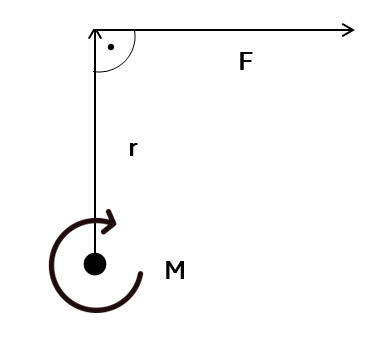
\includegraphics[width=7cm]{../ref/Drehmoment.png}
	\caption{Das Drehmoment visualisiert}
	\label{fig:mechanische-moment}
\end{figure}

Um das mechanische Drehmoment in beliebigen Lagen zu berechnen werden einige zusätzliche Informationen benötigt, wie die Masse und der Massenmittelpunkt der Konstruktion.

\begin{figure}[h!]
	\centering
	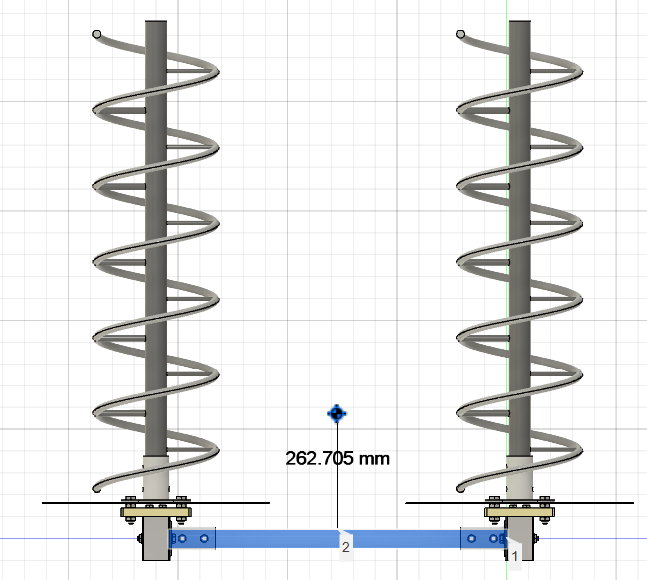
\includegraphics[width=7cm]{../ref/Massenmittelpunkt.png}
	\caption{Das Massenzentrum der Konstruktion}
	\label{fig:massenmittelpunkt}
\end{figure}

Es ist ersichtlich, dass sich der Massenmittelpunkt 262,705mm über dem oberen Ende des Strukturrohres befindet. Um daraus folgt, dass der Massenmittelpunkt $\frac{42mm}{2}+262,705mm=283,705mm$ über dem Mittelpunkt des Rotors befindet. Die Masse der Gesamtkonstruktion beträgt 23,32kg.

Aus diesen Informationen lässt sich nun das benötigte Moment für das Bewegen des Rotors in verschiedenen Lagen berechnen.

Der Hersteller des Rotors hat für den Stellungswinkel des Elevationsmotors die Reichweite 0-180° festgelegt. Um den Stellungswinkel direkt in Formel \ref{form:drehmoment} einsetzen zu können, müssen entweder 90° des Winkels abgezogen werden, oder der $-\cos(\alpha)$ verwendet werden. Hier wurde letztere Methode angewendet.

\begin{equation}
	M=F*r*(-\cos(\alpha))
\end{equation}

Nun kann ein Graph erzeugt werden, welcher das benötigte Moment in Abhängigkeit der Elevationsmotor-Stellung darstellt. Es ist anzumerken, dass die Effekte des Trägheitsmoments nicht berücksichtigt werden. Negative Werte repräsentieren das Drehmoment in die entgegengesetzte Richtung.

\begin{figure}[h!]
	\centering
	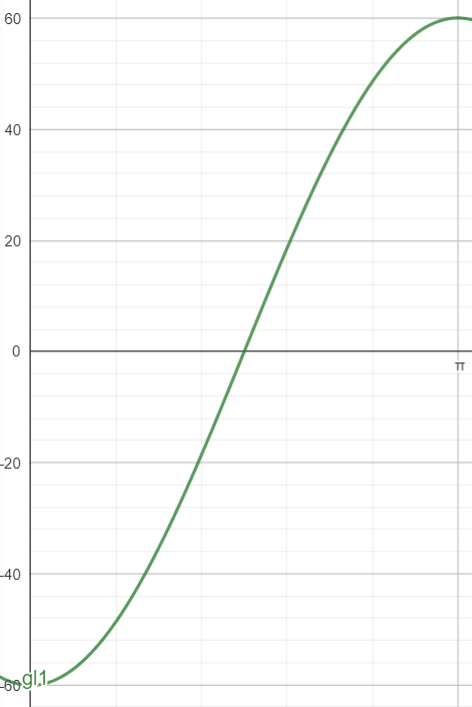
\includegraphics[width=5cm]{../ref/Rotationsmoment Elevation.png}
	\caption{Verlauf des Drehmoments über die Winkel 0-180°}
	\label{fig:verlauf-drehmoment}
\end{figure}

Es ist zu erwarten, dass das benötigte Rotationsmoment dann maximal ist, wenn der Rotor im 0° bzw. 180° Winkel steht. 
\begin{equation}
	M=23,32kg*9,81\frac{m}{s^2}*0,262705m*\sin(90°)=60,1Nm
\end{equation}

\begin{figure}[H]
	\begin{minipage}[b]{.4\linewidth} % [b] => Ausrichtung an \caption
		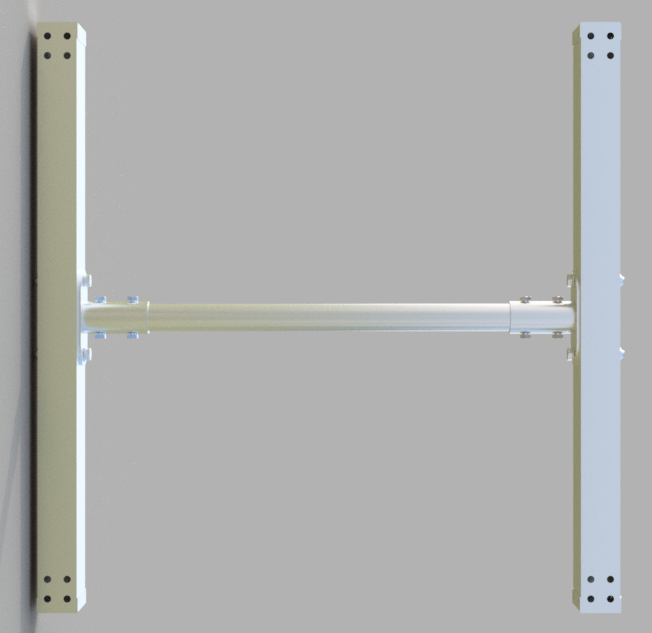
\includegraphics[width=\linewidth]{../ref/0000-Gesamtbaugruppe_Rahmen.png}
		\label{fig:Gerüst-Zeichnung}
	\end{minipage}
	\hspace{.1\linewidth}% Abstand zwischen Bilder
	\begin{minipage}[b]{.4\linewidth} % [b] => Ausrichtung an \caption
		\includegraphics[width=\linewidth]{../ref/Gerüst.jpg}
		\label{fig:Gerüst-real}
	\end{minipage}
	\caption{Gegenüberstellung des Renders zum realen Gerüst. In der realen Konstruktion sind bereits Teflonplatten montiert.}
\end{figure}

Um eine komplette elektrische Isolierung der Antennen vom Gerüst zu ermöglichen, kommen Teflonplatten zum Einsatz. Diese verbinden die Antennen mit dem Aluminium-Vierkantprofil.

\begin{figure}[H]
	\centering
	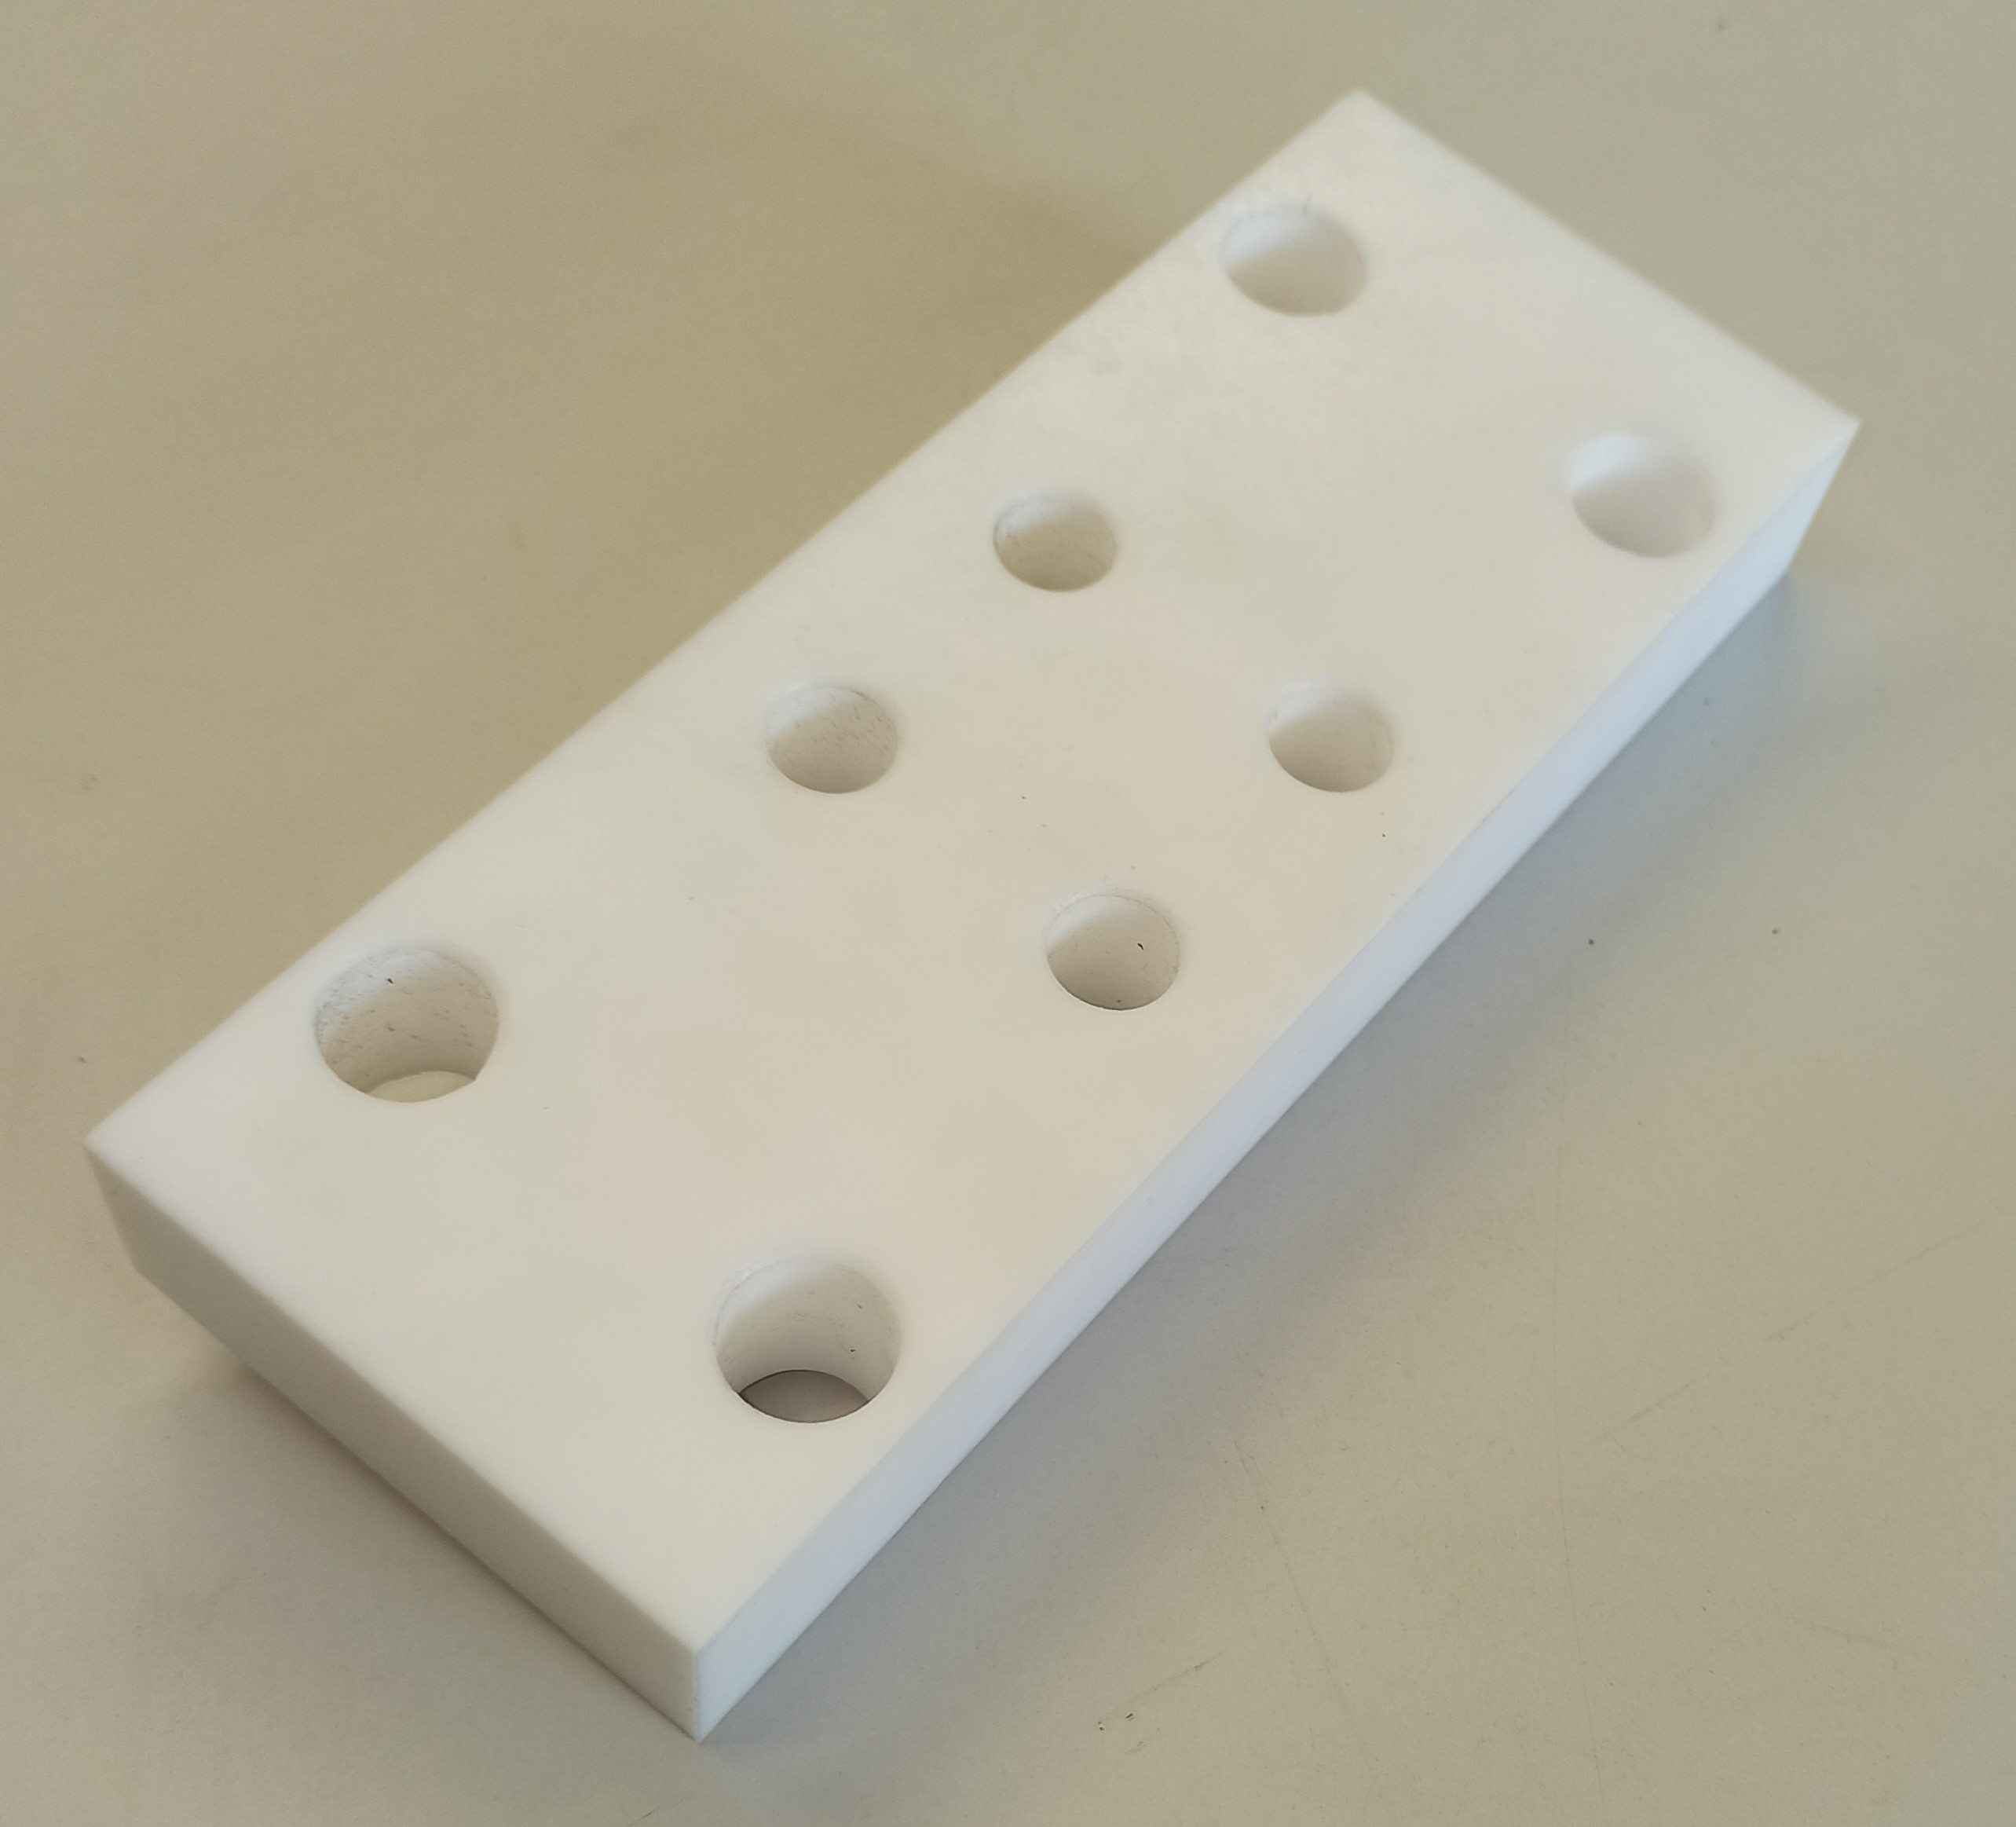
\includegraphics[width=5cm]{../ref/Teflon-Platte.jpg}
	\caption{Verbindende Teflonplatte}
	\label{fig:Teflonplatte}
\end{figure}

\subsection{Anpassung}
Da sich der Eingangswiderstand ändert, wenn vier solcher Antennen zusammen geschaltet werden, muss ein Anpassungsglied zwischen Koaxialkabel und Antennen eingesetzt werden. Hierfür wird ein $\lambda/4$-Anpasstopf gebaut. Dieser verhält sich ähnlich wie ein Koaxialkabel, wobei das Verhältnis der Durchmesser zwischen Innenleiter und Außenleiter die Kapazität festlegt. Hierdurch kann der Wellenwiderstand angepasst werden.

\begin{figure}[H]
	\centering
	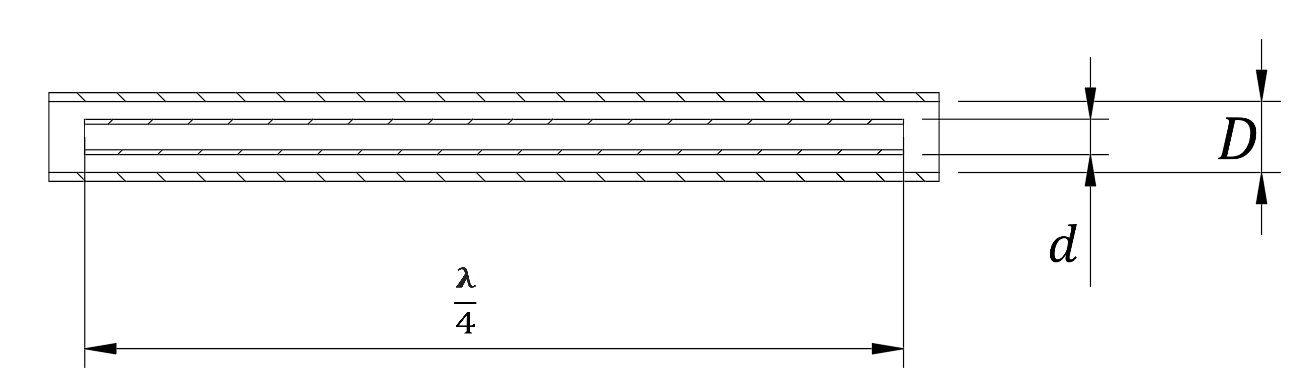
\includegraphics[width=\textwidth]{../ref/Prinzip-Anpasstopf.png}
	\label{fig:prinzip-anpasstopf}
	\caption{Querschnitt einer $\frac{\lambda}{4}$-Anpassleitung}
\end{figure}

Hierbei ist d der äußere Durchmesser des Innenleiters und D der innere Durchmesser des Außenleiters. Der Innenleiter ist $\frac{\lambda}{4}$ lang.

Für eine verlustlose $\frac{\lambda}{4}$-Leitung gilt:
\begin{equation}
	Z_E=\frac{(Z_W)^2}{Z_A}	
\end{equation}

Wobei $Z_E$ Der Eingangswiderstand des Anpasstopfes ist, $Z_A$ der Abschlusswiderstand und $Z_W$ der Wellenwiderstand der $\frac{\lambda}{4}$ Leitung \cite{admin_lambda4_2016}.

Um die Leitung korrekt zu dimensionieren muss zuerst der Wellenwiderstand ermittelt werden. Alle vier Helixantennen haben einen Antennenwiderstand von ca. 50$\Omega$. Werden diese parallel geschalten, so ergibt sich ein Gesamtwiderstand von 12,5$\Omega$. Da ein Koaxialkabel mit einem Wellenwiderstand von 50$\Omega$ verwendet wird, ist der Widerstand $Z_E$ 50$\Omega$. Somit ergibt sich durch umformen auf den Wellenwiderstand und einsetzen der Werte das nachfolgende Ergebnis \cite{admin_lambda4_2016}.

\begin{equation}
	Z_W=\sqrt{Z_E*Z_A}=\sqrt{12,5\Omega*50\Omega}=25\Omega
\end{equation}

Nun kann die Leitung dimensioniert werden. Es wurde ein viereckiger Außenleiter gewählt, da dies die Montage der BNC-Stecker vereinfacht. Um die Maße für die Leitung zu ermitteln, muss zuerst entweder der Durchmesser des Außenleiters oder des Innenleiters angenommen werden. Da ein 20x1.5mm Vierkantprofil verfügbar war, wurde dies als Außenleiter angenommen. Da der Innendurchmesser des Vierkantrohrs für die Kapazität relevant ist, wird $D=20mm-2*1,5mm=17mm$ gewählt. Daraus folgt für den Innenleiter:

\begin{equation}
	d=\frac{1,08*D}{10^{\frac{Z_W}{138}}}=\frac{1,08*17}{10^{\frac{25}{138}}}=12,09mm
\end{equation}


Es wird ein Kupferrohr mit einem Durchmesser von 12mm gewählt \cite{admin_lambda4_2016}.

Da die Maße feststehen, kann der Anpasstopf konstruiert werden. Es wurden als Addition Abdeckungen 3D-gedruckt.

\begin{figure}[H]
	\centering
	\begin{minipage}[b]{.2\linewidth} % [b] => Ausrichtung an \caption
		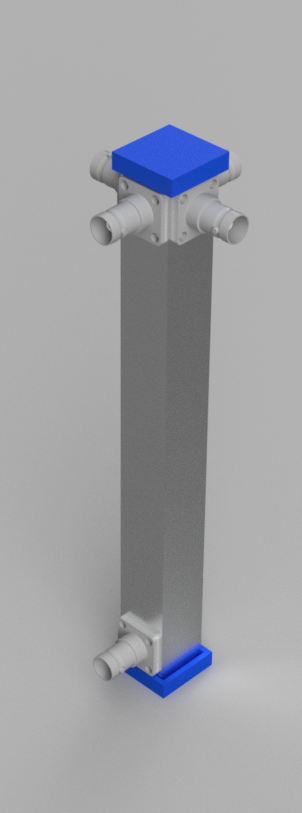
\includegraphics[width=\linewidth]{../ref/Lambda_4-Anpasstopf v1.png}
		\label{fig:Anpassleitung-Render}
	\end{minipage}
	\hspace{.1\linewidth}% Abstand zwischen Bilder
	\begin{minipage}[b]{.2\linewidth} % [b] => Ausrichtung an \caption
		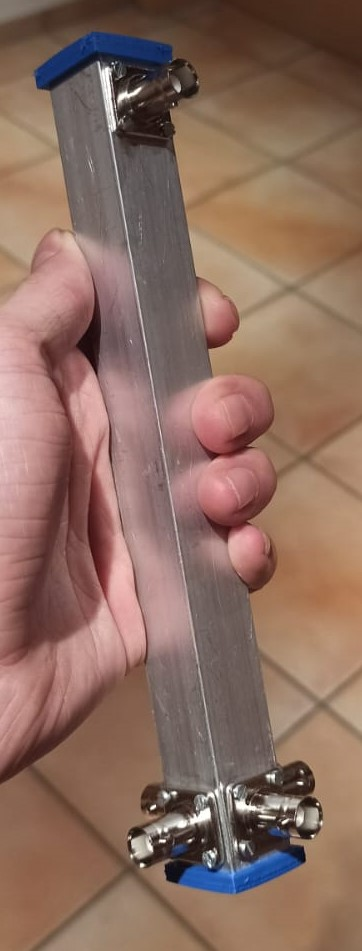
\includegraphics[width=\linewidth]{../ref/Anpasstopf-real.jpeg}
		\label{fig:Anpassleitung-real}
	\end{minipage}
	\caption{Gegenüberstellung des Renders zur realen Anpassleitung}
\end{figure}

\subsection{Messungen}
Um die Qualität des Antennenarrays zu überprüfen, wurde am Ausgang der $\frac{\lambda}{4}$-Anpassleitung gemessen. Hierbei werden der S11-Parameter, das SWR sowie das Smith-Diagramm analysiert, um qualitativ festzustellen, ob das Antennenarray funktionsfähig ist.

\begin{figure}[H]
	\centering
	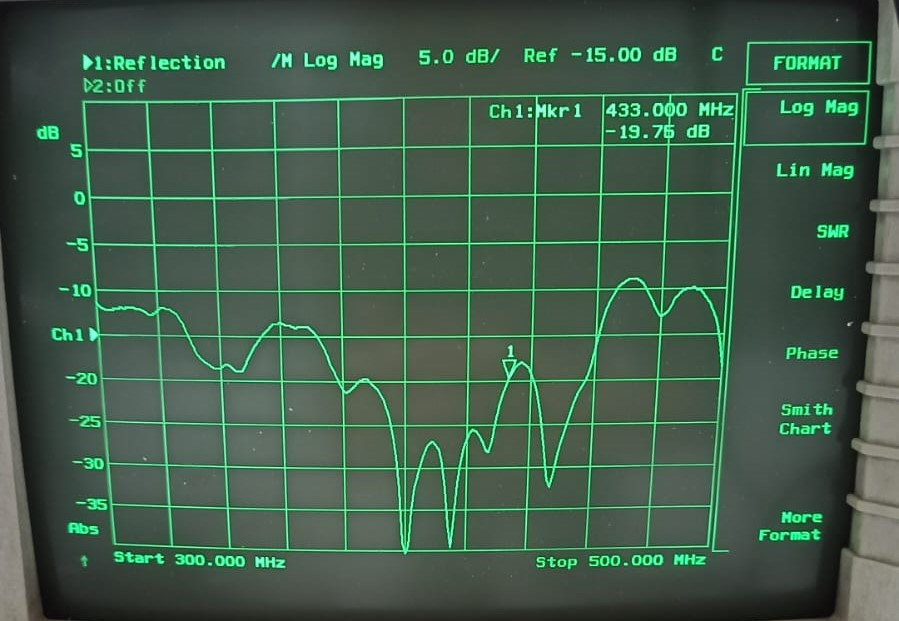
\includegraphics[width=10cm]{../ref/Array-S11.jpg}
	\label{fig:array-S11}
	\caption{S11-Parameter des Arrays}
\end{figure}

Anhand des S11-Parameters lässt sich feststellen, dass dieser mit einem Wert von ca. -20dB in einem relativ guten Bereich liegt.

\begin{figure}[H]
	\centering
	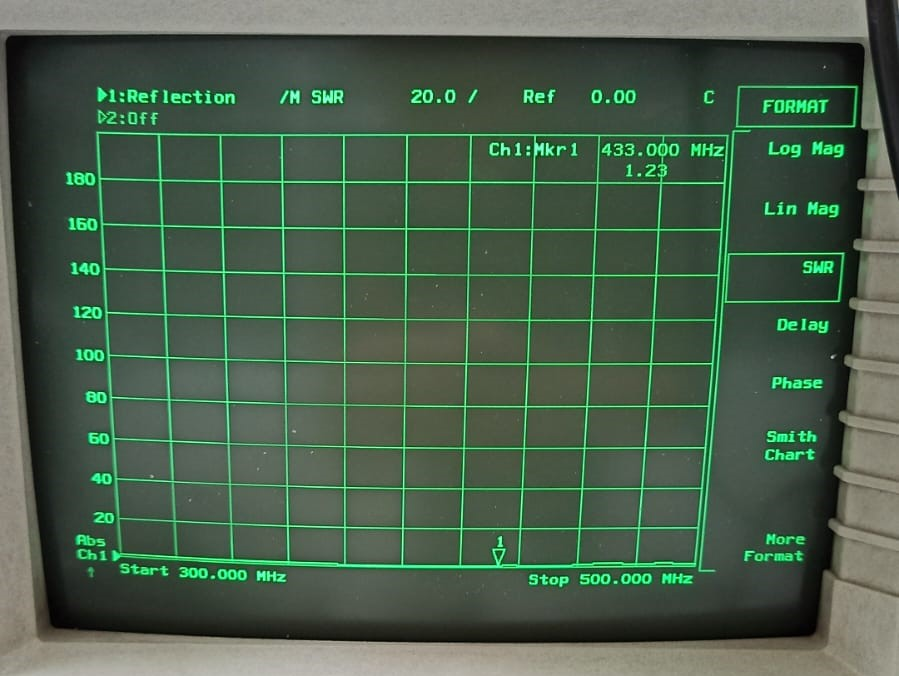
\includegraphics[width=10cm]{../ref/Array-SWR.jpg}
	\label{fig:array-SWR}
	\caption{SWR des Arrays}
\end{figure}

Mithilfe des SWRs kann ebenfalls auf die Güte der Anpassung geschlossen werden. Hier liegt der Wert ungefähr bei 1,2, was ein akzeptabler Wert ist.

\begin{figure}[H]
	\centering
	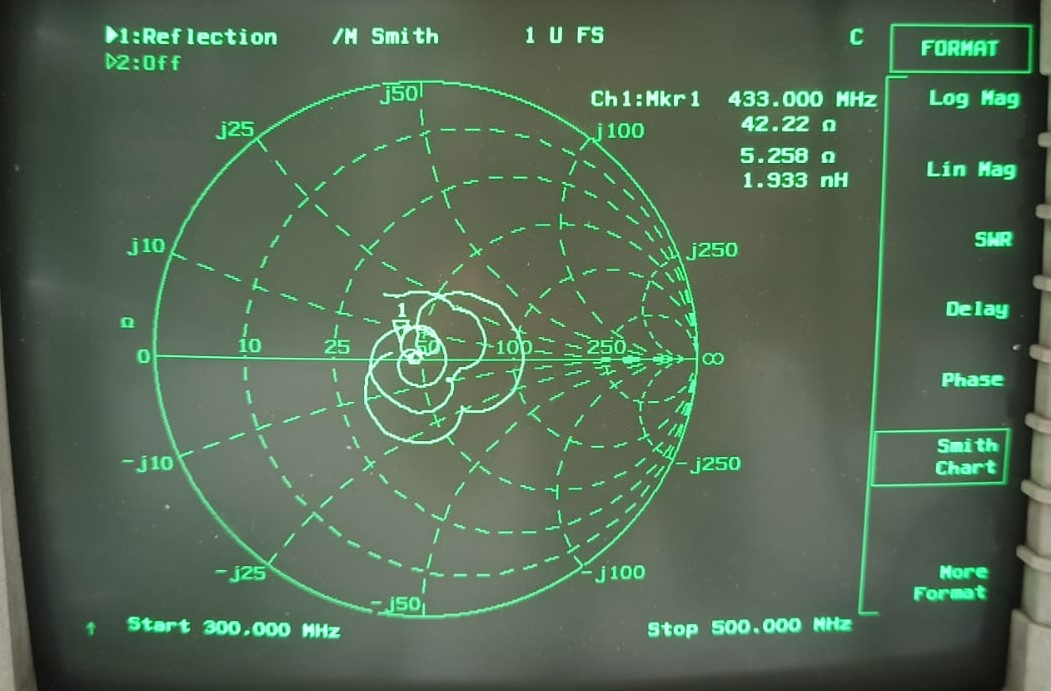
\includegraphics[width=10cm]{../ref/Array-Smith.jpg}
	\label{fig:array-Smith}
	\caption{Smith-Diagramm des Arrays}
\end{figure}

Am Smith-Diagramm ist zu erkennen, dass die Eingangsimpedanz der Antenne kaum imaginär ist und mit 42 Ohm relativ gut im Mittelpunkt des Smith-Diagramms liegt.

\section{Test}
Um die Funktionalität des Helix-Arrays und des Rotors nachzuweisen, wurden mehrere Observationen durchgeführt. Dabei wurden die Signale der einzelnen Helix-Antennen mithilfe des $\lambda/4$-Anpasstopfes zu einem Signal zusammengeführt.

Die Observationen wurden am 16. März 2024, an den Koordinaten 47.27139319984484, 9.63248486985336 (Negrellistraße 50, 6830 Rankweil), auf einer Höhe von 459 Metern über dem Meeresspiegel, durchgeführt.  Die Ergebnisse der Observationen, die zum Test der Funktionalität durchgeführt wurden, können unter folgendem Link aufgerufen werden:\newline \url{https://network.satnogs.org/observations/?norad=&start=2024-03-16+00%3A01&end=2024-03-17+20%3A59&observer=&station=3307&transmitter_mode=&transmitter_uuid=}

Mit 29 empfangenen Paketen empfing die Observation mit der Nummer 9209920 des Satelliten \glqq 53106 - GREENCUBE\grqq{}  und dem Sender \glqq Mode U TLM 1k2 GMSK\grqq{} die meisten Datenpakete. Die Daten wurden am 16. März 2024 von 13:39:27 bis 13:51:27 (UTC) empfangen. Die nachfolgende Abbildung zeigt das Wasserfalldiagramm sowie das erste dekodierte Datenpaket im HEX und ASCII Format.

\begin{figure} [H]
	\centering
	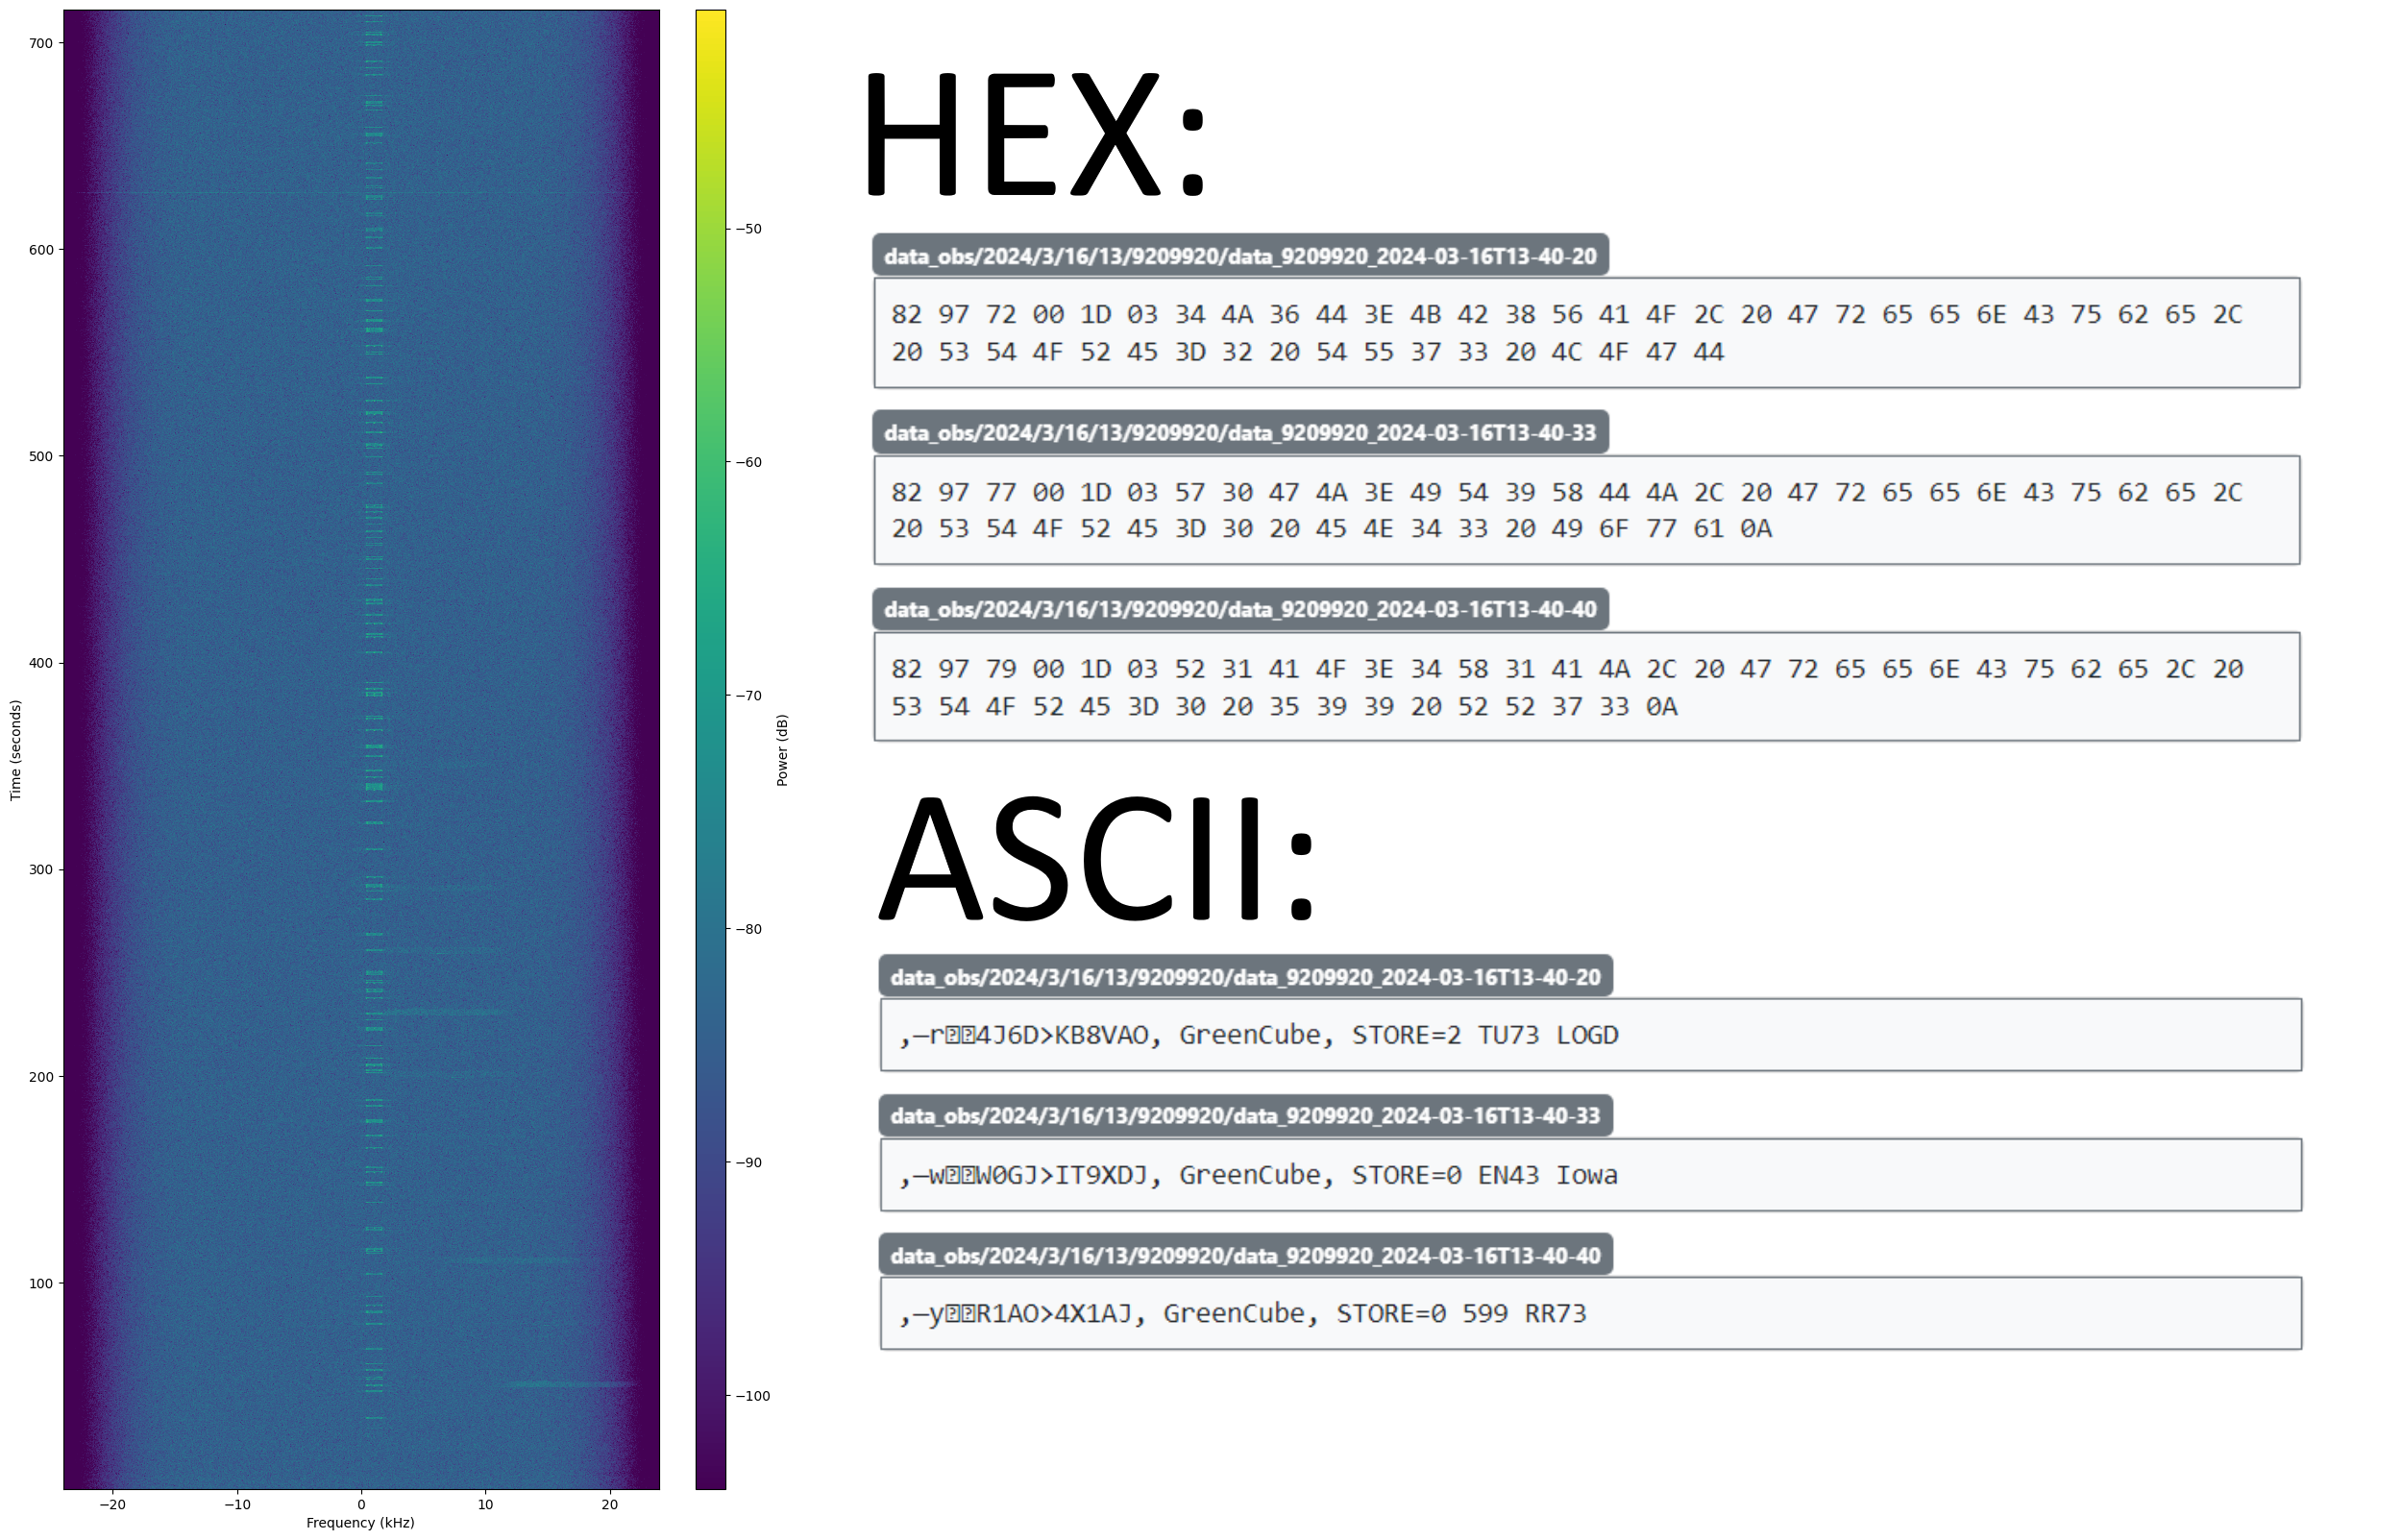
\includegraphics[width=\linewidth]{../ref/helix_successfull_observation.png}
	\caption{Wasserfalldiagramm und erstes Datenpaket in HEX und ASCII Format der Observation 9209920 \cite{noauthor_satnogs_observation_helix_nodate}}
	\label{fig:helix_successfull_observation}
\end{figure}